%%%%%%%%%%%%%%%%%%%%%%%%%%%%%%%%%%%%%%%%%%%%%%%%%%%%%%%%%%%%%%%%%%%%%%%%%%%%%%%%
%2345678901234567890123456789012345678901234567890123456789012345678901234567890
%        1         2         3         4         5         6         7         8

% \documentclass[letterpaper, 10 pt, conference]{ieeeconf}  % Comment this line out if you need a4paper

\documentclass[a4paper, 10pt, conference]{ieeeconf}      % Use this line for a4 paper
    
\IEEEoverridecommandlockouts                              % This command is only needed if 
                                                          % you want to use the \thanks command

\overrideIEEEmargins                                      % Needed to meet printer requirements.

%In case you encounter the following error:
%Error 1010 The PDF file may be corrupt (unable to open PDF file) OR
%Error 1000 An error occurred while parsing a contents stream. Unable to analyze the PDF file.
%This is a known problem with pdfLaTeX conversion filter. The file cannot be opened with acrobat reader
%Please use one of the alternatives below to circumvent this error by uncommenting one or the other
%\pdfobjcompresslevel=0
%\pdfminorversion=4

% See the \addtolength command later in the file to balance the column lengths
% on the last page of the document

% The following packages can be found on http:\\www.ctan.org
\usepackage{graphics} % for pdf, bitmapped graphics files
%\usepackage{epsfig} % for postscript graphics files
%\usepackage{mathptmx} % assumes new font selection scheme installed
%\usepackage{times} % assumes new font selection scheme installed
\usepackage{amsmath} % assumes amsmath package installed
\usepackage{amssymb}  % assumes amsmath package installed
\usepackage{tikz}
\usepackage{float}
% \usepackage{caption}
\usetikzlibrary{shapes.geometric, arrows.meta, positioning, fit, calc}
\newcommand{\hdr}{\scriptsize\itshape\bfseries}   % heading style used inside the architecture figure
\usepackage{bm}
\usepackage{graphicx}  
\usepackage{hyperref}
% \usepackage{fancyhdr}
% \usepackage{natbib}  




\title{\LARGE \bf
MERLIN - Multi-arm Experimental Robotics Learning and INtegration
}
\author{Saipushkar Nagaraj$^{1}$, Yash Sanjeev Halbhavi$^{2}$ and Ameer K. Mulla$^{3}$% <-this % stops a space
\thanks{$^{1}$This work is partially supported by Anusandhan National Research Foundation (ANRF), Govt. of India}%
\thanks{$^{2}$A Video demonstration of the Testbed is available at \url{https://youtu.be/_An5y608v_o}}
}


\begin{document}



\maketitle
\thispagestyle{empty}
\pagestyle{empty}


%%%%%%%%%%%%%%%%%%%%%%%%%%%%%%%%%%%%%%%%%%%%%%%%%%%%%%%%%%%%%%%%%%%%%%%%%%%%%%%%
\begin{abstract}
Modern robotic arm research needs a single platform for hybrid simulation-to-hardware execution, reinforcement learning (RL) data collection, camera-geometry-aware policy training, and bilateral teleoperation. This paper presents MERLIN, a robotic arm testbed that combines bilateral teleoperation, multi-arm interoperability, an in-GUI environment for developing and tuning control laws (with MATLAB), and a geometry-aware data-collection pipeline in one software architecture. The platform records camera intrinsics, extrinsics, and ray embeddings together with joint states, motor currents, and commanded actions in a unified episode schema. For force-reflecting teleoperation without force sensors, a ReactorX 200 / ViperX 300S pair uses a momentum-observer force estimate, an exactly discretised admittance, a constrained offset-free MPC for position-controlled slaves, and an energy-tank passivity guard. On the real arms, the initial implementation reached an overall tracking RMSE of 0.358\,rad. The revised controller is evaluated in a MuJoCo model of the same arms, where it lowers free-motion tracking error from 0.22 to 0.007\,rad and reproduces applied forces at the master (correlation 0.94--0.98); its measurement on hardware is outstanding.

\end{abstract}


%%%%%%%%%%%%%%%%%%%%%%%%%%%%%%%%%%%%%%%%%%%%%%%%%%%%%%%%%%%%%%%%%%%%%%%%%%%%%%%%
\section{Introduction}

% This template provides authors with most of the formatting specifications needed for preparing electronic versions of their papers. All standard paper components have been specified for three reasons: (1) ease of use when formatting individual papers, (2) automatic compliance to electronic requirements that facilitate the concurrent or later production of electronic products, and (3) conformity of style throughout a conference proceedings. Margins, column widths, line spacing, and type styles are built-in; examples of the type styles are provided throughout this document and are identified in italic type, within parentheses, following the example. Some components, such as multi-leveled equations, graphics, and tables are not prescribed, although the various table text styles are provided. The formatter will need to create these components, incorporating the applicable criteria that follow.

Robotic arm teleoperation and control remain central to applications such as surgery, hazardous manipulation, space exploration, and industrial automation. Progress in bilateral teleoperation, reinforcement learning (RL), and hybrid sim-to-real workflows now requires platforms that span the full research lifecycle, from controller prototyping to large-scale data collection.

Deep RL has produced strong manipulation policies \cite{han2023deeprl, singh2019endtoend}, but performance depends on data quality and scale, and thus on reliable teleoperation, synchronized multi-sensor logging, and safe experimental infrastructure \cite{mahmood2018senseact}. Viewpoint generalization is an added difficulty: visual policies often latch onto static background cues instead of geometry-aware features \cite{jiang2025kyknow}.

To our knowledge, no existing system unifies bilateral teleoperation, custom control, RL data collection, camera-geometry logging, and hybrid sim-real operation. Researchers therefore maintain separate stacks, which slows development and weakens reproducibility. MERLIN closes this gap with a single extensible testbed and a consistent data model, so effort can go to algorithms rather than integration.

% Robotic arm teleoperation and control remain central challenges in robotics research, with applications spanning surgical intervention, hazardous environment manipulation, space exploration, and industrial automation \cite{surgicalRobotics}. The convergence of bilateral teleoperation, reinforcement learning (RL), and hybrid simulation-real workflows has created a demand for unified experimental platforms that can support the full lifecycle of robotic arm research, from controller prototyping to large-scale data collection. 

% Recent advances in deep RL for manipulation have demonstrated that learning-based policies can achieve impressive performance on complex tasks \cite{han2023deeprl, singh2019endtoend}. However, these results depend critically on the quality and scale of training data, which in turn depends on the availability of reliable teleoperation interfaces, synchronized multi-sensor logging, and safe experimentation infrastructure \cite{mahmood2018senseact}. The challenge is compounded when policies must generalize across camera viewpoints, as visual policies often exploit static background cues rather than learning geometry-aware representations \cite{jiang2025kyknow}.

% Simultaneously, the robotics community has recognized that no single existing platform provides a unified environment that seamlessly integrates bilateral teleoperation, custom control development, RL data collection, camera geometry logging, and hybrid simulation-real operations. This fragmentation forces researchers to maintain separate systems for each capability, increasing development time and reducing reproducibility. 
% MERLIN addresses this gap by providing a single, extensible testbed that unifies all of these capabilities under a consistent data model. This unified design allows researchers to focus on algorithm development rather than software integration, thereby accelerating research in robotic manipulation, bilateral teleoperation, and autonomous control.

% \section{Related Work and Limitations of Existing Approaches}
% % \vspace{-0.25cm}
% \subsection{Bilateral Teleoperation and Force Feedback}
% % \vspace{-0.25cm}
% Existing bilateral teleoperation systems have made significant progress in achieving transparent force feedback and stable control. \cite{MPCcontroller} proposed a four-channel bilateral teleoperation framework unifying impedance and admittance control for dual-arm systems, enabling force feedback from both the arm and gripper.\cite{articleminetal} introduced a two-layer architecture separating passivity guarantees from transparency design through shared energy tanks, validated on the da Vinci research kit \cite{davinci}. These works demonstrate that modern teleoperation systems can achieve high fidelity; however, they are typically designed for a single control paradigm and do not natively support the heterogeneous workflows required by contemporary robotics research.

% \subsection{Scalable Data Collection and Teleoperation Platforms}
% % \vspace{-0.25cm}
% Platforms for RL data collection have advanced considerably. \cite{10759864} developed a twin dual-arm testbed for consistent human demonstration data collection, where a leader robot duplicates the operator's actions onto a follower robot via ROS2 communication. \cite{unibidex} presented a unified teleoperation framework supporting both VR and leader-follower input modalities with null-space control for collision-free bimanual manipulation.\cite{dass2023pato} introduced policy-assisted teleoperation that automates repetitive subtasks using a hierarchical assistive policy, enabling a single operator to control multiple robots simultaneously and significantly improving data collection throughput. OPEN TEACH \cite{iyer2024openteach} provided a VR-based plug-and-play teleoperation system supporting multiple robot morphologies at 90 Hz, while \cite{wu2023gello} demonstrated a low-cost, 3D-printable teleoperation framework for Franka, UR5, and xArm with superior task success rates compared to VR controllers and spacemouse devices. \cite{mandlekar2019roboturk} scaled remote teleoperation to over 111 hours of manipulation data across 54 users in one week, and Mobile ALOHA \cite{fu2024mobilealoha} demonstrated that co-training with existing static datasets can boost mobile manipulation success rates by up to 90\%. While these systems address data collection effectively, they are specialized for either teleoperation or learning, and do not provide integrated support for custom control algorithm development, parameter optimization, or hybrid simulation-real experimentation within a single platform.

% % \subsection{Multi-Embodiment Datasets and Standardized Benchmarks}
% % The importance of standardized, large-scale datasets has been demonstrated by several recent efforts. RoboMIND \cite{wu2024robomind} introduced a dataset of 107k demonstration trajectories across 4 robotic embodiments, 479 tasks, and 96 object classes, collected on a unified platform with multi-view cameras, proprioceptive state, and language descriptions. Open X-Embodiment \cite{openxembodiment2023} assembled a dataset from 22 robots across 21 institutions, demonstrating that high-capacity models trained on diverse cross-robot data exhibit positive transfer. DROID \cite{khazatsky2024droid} provided a large-scale in-the-wild manipulation dataset. These works establish that dataset quality and standardization are essential for generalizable policy learning, but they focus on dataset creation rather than on providing an integrated platform for simultaneous control development and data collection.

% \subsection{Reinforcement Learning for Robotic Manipulation}
% % \vspace{-0.25cm}
% The application of RL to robotic manipulation has grown rapidly \cite{
% han2023deeprl, mahmood2018senseact} provided foundational guidelines for real-world RL setup, demonstrating that learning performance is highly sensitive to delays, action cycle timing, and action representation. \cite{singh2019endtoend} showed that end-to-end RL from camera images can learn manipulation tasks without manually engineered reward functions. \cite{zhu2018visuomotor} combined RL with imitation learning to train visuomotor policies mapping RGB camera inputs directly to joint velocities, achieving zero-shot sim-to-real transfer. \cite{endrawis2021efficient} proposed active data collection using goal-conditioned RL to produce diverse datasets for offline learning. These works highlight the importance of well-designed experimentation infrastructure, yet none provide a unified platform that integrates control development, data collection, and hybrid simulation-hardware execution.

% \subsection{Camera Geometry and Viewpoint Generalization}
% % \vspace{-0.25cm}
% A persistent challenge in vision-based robot learning is viewpoint generalization. \cite{jiang2025kyknow} showed that explicitly conditioning policies on camera intrinsics and extrinsics, using Pl\"{u}cker ray embeddings, significantly improves generalization across viewpoints for standard behavior cloning policies including ACT, Diffusion Policy, and SmolVLA. Their analysis reveals that policies without extrinsics conditioning exploit static background cues as shortcuts, which collapse when camera placement or workspace geometry shifts. \cite{wei2024maniwhere} proposed a visual generalization framework for RL that uses multi-view representation learning with a Spatial Transformer Network (STN) module and curriculum-based domain randomization, demonstrating strong sim-to-real transfer across three hardware platforms. \cite{lee2020dream} addressed camera-to-robot pose estimation from a single RGB image using deep learning and PnP, enabling online calibration without offline hand-eye procedures. These works establish that camera geometry awareness is critical for robust visual policies, yet existing robotic platforms do not natively capture and store camera calibration data alongside robot state.

% \subsection{Digital Twins and MATLAB-Based Control}
% % \vspace{-0.25cm}
% Digital twin approaches have been explored for robotic arm control. \cite{cen2025digitaltwin} presented a digital twin-empowered system combining proximal policy optimization (PPO) with fuzzy PID for virtual-real mapping error correction. On the classical control side, \cite{iqbal2019matlab} demonstrated H-infinity and model predictive control (MPC) design for robotic manipulators using MATLAB/Simulink showcasing the importance of systematic fine-tuning in simulation before deployment, while\cite{chaos2013virtual} built a virtual and remote robotic laboratory using MATLAB and LabVIEW with a unified GUI for simulation and real-robot experimentation. These works show the value of integrating simulation, classical control, and MATLAB-based analysis, but they do not combine these capabilities with modern RL data collection or camera geometry logging.
% The comprehensive review by \cite{surgicalRobotics} highlights that recent research has shifted from basic motion synchronization to complex, stability-oriented architectures incorporating virtual reality, AI-driven force prediction, and multi-sensor fusion. But lack a unified environment that seamlessly integrates bilateral teleoperation, custom control development, RL data collection, camera geometry-aware logging, and hybrid simulation-real operations under a single software architecture.

% \section{PROCEDURE FOR PAPER SUBMISSION}

% \subsection{Selecting a Template (Heading 2)}

% First, confirm that you have the correct template for your paper size. This template has been tailored for output on the US-letter paper size. 
% It may be used for A4 paper size if the paper size setting is suitably modified.

% \subsection{Maintaining the Integrity of the Specifications}

% The template is used to format your paper and style the text. All margins, column widths, line spaces, and text fonts are prescribed; please do not alter them. You may note peculiarities. For example, the head margin in this template measures proportionately more than is customary. This measurement and others are deliberate, using specifications that anticipate your paper as one part of the entire proceedings, and not as an independent document. Please do not revise any of the current designations



\section{Contribution}
% \vspace{-0.35cm}
This paper presents MERLIN, a comprehensive robotic arm control testbed designed to serve as a unified research platform addressing the aforementioned limitations. The system has the following architecture layout along with the following features:

\vspace{-0.3cm}
\subsection{System Architecture}
\vspace{-0.215cm}
The MERLIN architecture is organized as a layered stack consisting of five core modules, all unified through a shared calibration, synchronization, and safety layer. \\Fig. \ref{fig:architecture}. presents the high-level system architecture.



% \begin{figure}[t]
% \centering
% \setlength{\mblockw}{\columnwidth-1.75cm\relax} % main stack width
% \setlength{\mmodew}{0.20\columnwidth\relax}     % execution-mode width
% \begin{tikzpicture}[
%     every node/.style={font=\scriptsize},
%     block/.style={
%         rectangle, draw, thick, rounded corners,
%         align=center, fill=white, inner sep=3pt
%     },
%     arrow/.style={thick, -{Latex[scale=0.7]}}
% ]

% % ---- Stage 2: five modules ----
% \node[block, text width=\mblockw] (multiarm)
%   {\textit{\textbf{Multi-Arm Support}}\\[1pt]
%    \textbf{1.} Visualization (RViz) \quad \textbf{2.} Motor Status};

% \node[block, text width=\mblockw, below=0.18cm of multiarm] (mpc)
%   {\textit{\textbf{MPC Force Feedback Controller}}};

% \node[block, text width=\mblockw, below=0.18cm of mpc] (matlab)
%   {\textit{\textbf{MATLAB Integration}}\\[1pt]
%    \textbf{1.} Algorithm Verification \quad \textbf{2.} Parameter Tuning};

% \node[block, text width=\mblockw, below=0.18cm of matlab] (rl)
%   {\textit{\textbf{RL Data Procurement Pipeline}}};

% \node[block, text width=\mblockw, below=0.18cm of rl] (teleop)
%   {\textit{\textbf{Teleoperation}}\\[1pt]
%    \textbf{1.} Direct Joint Control \quad \textbf{2.} Joystick \quad \textbf{3.} Camera (WebXR)};

% % ---- Stage 1: GUI ----
% \node[block, text width=\mblockw, above=0.85cm of multiarm] (gui)
%   {\textit{\textbf{GUI / Unified Interface Layer}}};

% % ---- Left bus: GUI -> all modules ----
% \coordinate (lbus) at ([xshift=-0.5cm]multiarm.west);
% \draw[thick] (gui.south) -- ++(0,-0.32) -| (multiarm.west -| lbus);
% \draw[thick] (multiarm.west -| lbus) -- (teleop.west -| lbus);
% \draw[arrow] (multiarm.west -| lbus) -- (multiarm.west);
% \draw[arrow] (mpc.west      -| lbus) -- (mpc.west);
% \draw[arrow] (matlab.west   -| lbus) -- (matlab.west);
% \draw[arrow] (rl.west       -| lbus) -- (rl.west);
% \draw[arrow] (teleop.west   -| lbus) -- (teleop.west);

% % ---- Stage 3: calibration / synchronization / safety ----
% \node[block, fill=gray!10, text width=\mblockw, below=1.0cm of teleop] (cal)
%   {\textit{\textbf{Calibration, Synchronization \& Safety Layer}}\\[1pt]
%    Camera intrinsics \quad extrinsics \quad ray embeddings \quad joint sync \quad E-stop};

% % ---- Right bus: all modules -> calibration ----
% \coordinate (rbus)  at ([xshift=0.5cm]multiarm.east);
% \coordinate (rbot)  at (teleop.east -| rbus);
% \coordinate (rjoin) at ([yshift=-0.42cm]rbot);
% \draw[thick] (multiarm.east) -- (multiarm.east -| rbus);
% \draw[thick] (mpc.east)      -- (mpc.east      -| rbus);
% \draw[thick] (matlab.east)   -- (matlab.east   -| rbus);
% \draw[thick] (rl.east)       -- (rl.east       -| rbus);
% \draw[thick] (teleop.east)   -- (teleop.east   -| rbus);
% \draw[thick] (multiarm.east -| rbus) -- (rjoin);
% \draw[arrow] (rjoin) -| (cal.north);

% % ---- Stage 4: unified episode store ----
% \node[block, fill=blue!5, text width=\mblockw, below=0.45cm of cal] (store)
%   {\textit{\textbf{Unified Episode Store}}\\[1pt]
%    RGB \quad depth \quad joint angles \quad velocities \quad torques\\
%    tactile \quad haptic \quad actions \quad rewards};
% \draw[arrow] (cal.south) -- (store.north);

% % ---- Stage 5: execution modes ----
% \node[block, fill=yellow!5, text width=\mmodew, below=0.8cm of store] (hybrid)
%   {\textit{\textbf{Hybrid}}};
% \node[block, fill=green!5, text width=\mmodew, left=0.5cm of hybrid] (sim)
%   {\textit{\textbf{Simulation}}};
% \node[block, fill=red!5, text width=\mmodew, right=0.5cm of hybrid] (hw)
%   {\textit{\textbf{Hardware}}};

% \draw[arrow] (store.south) -- ++(0,-0.38) -| (sim.north);
% \draw[arrow] (store.south) -- ++(0,-0.38) -| (hw.north);
% \draw[arrow] (store.south) -- (hybrid.north);

% \end{tikzpicture}
% \caption{High-level architecture of MERLIN: the unified interface drives five experimental modules, all of which pass through a shared calibration, synchronization, and safety layer into a unified episode store consumed by three execution modes.}
% \label{fig:architecture}
% \end{figure}

% \begin{figure*}[t]
% \centering
% \resizebox{0.7\textwidth}{!}{%
% \begin{tikzpicture}[
%     node distance=0.12cm and 0.35cm,
%     every node/.style={font=\scriptsize},
%     block/.style={
%         rectangle, draw, thick, rounded corners,
%         align=center, fill=white, inner sep=3pt
%     },
%     blocktall/.style={
%         rectangle, draw, thick, rounded corners,
%         align=center, fill=white, inner sep=3pt
%     },
%     arrow/.style={thick, -{Latex[scale=0.7]}}
% ]

% % ---- Column 1: GUI ----
% \node[block, minimum height=4.2cm, text width=3.2em] (gui)
%   {\textit{\textbf{GUI /\\Unified\\Interface\\Layer}}};

% % ---- Column 2: Five modules ----
% \node[blocktall, text width=8.6em, right=0.7cm of gui, yshift=1.85cm] (multiarm)
%   {\textit{\textbf{Multi-Arm Support}}\\[1pt]
%    \textbf{1.} Visualization (RViz)\\
%    \textbf{2.} Motor Status};

% \node[block, text width=8.6em, below=of multiarm] (mpc)
%   {\textit{\textbf{MPC Force Feedback Controller}}};

% \node[blocktall, text width=8.6em, below=of mpc] (matlab)
%   {\textit{\textbf{MATLAB Integration}}\\[1pt]
%    \textbf{1.} Algorithm Verification\\
%    \textbf{2.} Parameter Tuning};

% \node[block, text width=8.6em, below=of matlab] (rl)
%   {\textit{\textbf{RL Data Procurement Pipeline}}};

% \node[blocktall, text width=8.6em, below=of rl] (teleop)
%   {\textit{\textbf{Teleoperation}}\\[1pt]
%    \textbf{1.} Direct Joint Control\\
%    \textbf{2.} Joystick\\
%    \textbf{3.} Camera (WebXR)};

% \draw[arrow] (gui.east) -- ++(0.22,0) |- (multiarm.west);
% \draw[arrow] (gui.east) -- ++(0.22,0) |- (mpc.west);
% \draw[arrow] (gui.east) -- ++(0.22,0) |- (matlab.west);
% \draw[arrow] (gui.east) -- ++(0.22,0) |- (rl.west);
% \draw[arrow] (gui.east) -- ++(0.22,0) |- (teleop.west);

% % ---- Column 3: Calibration / Safety ----
% \node[block, fill=gray!10, minimum height=4.2cm, text width=5.4em,
%       right=0.55cm of matlab] (cal)
%   {\textit{\textbf{Calibration,\\Synchronization\\\& Safety Layer}}\\[2pt]
%    Camera intrinsics\\
%    extrinsics\\
%    ray embeddings\\
%    joint sync\\
%    E-stop};

% \draw[arrow] (multiarm.east) -- ++(0.22,0) |- (cal.west);
% \draw[arrow] (mpc.east) -- ++(0.22,0) |- (cal.west);
% \draw[arrow] (matlab.east) -- ++(0.22,0) |- (cal.west);
% \draw[arrow] (rl.east) -- ++(0.22,0) |- (cal.west);
% \draw[arrow] (teleop.east) -- ++(0.22,0) |- (cal.west);

% % ---- Column 4: Episode Store ----
% \node[block, fill=blue!5, minimum height=4.2cm, text width=4.6em,
%       right=0.4cm of cal] (store)
%   {\textit{\textbf{Unified\\Episode Store}}\\[2pt]
%    RGB\\
%    depth\\
%    joint angles\\
%    velocities\\
%    torques\\
%    tactile\\
%    haptic\\
%    actions\\
%    rewards};

% \draw[arrow] (cal.east) -- (store.west);

% % ---- Column 5: Execution modes ----
% \node[block, fill=green!5, text width=4.4em, right=0.5cm of store, yshift=0.85cm] (sim)
%   {\textit{\textbf{Simulation}}};
% \node[block, fill=yellow!5, text width=4.4em, below=0.18cm of sim] (hybrid)
%   {\textit{\textbf{Hybrid}}};
% \node[block, fill=red!5, text width=4.4em, below=0.18cm of hybrid] (hw)
%   {\textit{\textbf{Hardware}}};

% \draw[arrow] (store.east) -- ++(0.18,0) |- (sim.west);
% \draw[arrow] (store.east) -- ++(0.18,0) |- (hybrid.west);
% \draw[arrow] (store.east) -- ++(0.18,0) |- (hw.west);

% \end{tikzpicture}%
% }
% \caption{High-level architecture of MERLIN, shown as a horizontal data flow.}
% \label{fig:architecture}
% \end{figure*}


% \begin{figure*}[t]
% \centering
% % \begin{tikzpicture}[
% %     node distance=0.45cm and 0.55cm,
% %     every node/.style={font=\scriptsize}
% % ]

% % % ---- Column 1: GUI (spans the height of the five modules) ----
% % \node[block, minimum height=5.6cm, text width=4em, font=\footnotesize] (gui) {\textbf{GUI / Unified Interface Layer}};

% % % ---- Column 2: Five main modules, stacked vertically, with sub-items folded in ----
% % \node[blocktall, text width=9.5em, right=of gui, yshift=2.75cm] (multiarm)
% %   {\textbf{\footnotesize Multi-Arm Support}\\[2pt] \textbf{1.} Visualization (RViz) \quad \textbf{2.} Motor Status};
% % \node[block, text width=9.5em, below=0.3cm of multiarm] (mpc) {\textbf{\footnotesize MPC Force Feedback Controller}};
% % \node[blocktall, text width=9.5em, below=0.3cm of mpc] (matlab)
% %   {\textbf{\footnotesize MATLAB Integration}\\[2pt] \textbf{1.} Algorithm Verification \quad \textbf{2.} Parameter Tuning};
% % \node[block, text width=9.5em, below=0.3cm of matlab] (rl) {\textbf{\footnotesize RL Data Procurement Pipeline}};
% % \node[blocktall, text width=9.5em, below=0.3cm of rl] (teleop)
% %   {\textbf{\footnotesize Teleoperation}\\[2pt] \textbf{1.} Direct Joint Control \\ \textbf{2.} Joystick \\ \textbf{3.} Camera (WebXR)};

% % % Arrows from GUI to each module (Right angle routing)
% % \draw[arrow] (gui.east) -- ++(0.25,0) |- (multiarm.west);
% % \draw[arrow] (gui.east) -- ++(0.25,0) |- (mpc.west);
% % \draw[arrow] (gui.east) -- ++(0.25,0) |- (matlab.west);
% % \draw[arrow] (gui.east) -- ++(0.25,0) |- (rl.west);
% % \draw[arrow] (gui.east) -- ++(0.25,0) |- (teleop.west);

% % % ---- Column 3: Unified Calibration / Safety Layer ----
% % \node[block, fill=gray!10, minimum height=5.6cm, text width=7em,
% %       right=0.9cm of matlab] (cal) {\textbf{\footnotesize Calibration, \\ Synchronization \& Safety Layer}\\[2pt] Camera intrinsics $+$ extrinsics $+$ ray embeddings $+$ joint sync $+$ E-stop};

% % % Arrows from modules to Calibration Layer (Right angle routing)
% % \draw[arrow] (multiarm.east) -- ++(0.45,0) |- (cal.west);
% % \draw[arrow] (mpc.east) -- ++(0.45,0) |- (cal.west);
% % \draw[arrow] (matlab.east) -- ++(0.45,0) |- (cal.west);
% % \draw[arrow] (rl.east) -- ++(0.45,0) |- (cal.west);
% % \draw[arrow] (teleop.east) -- ++(0.45,0) |- (cal.west);

% % % ---- Column 4: Unified Episode Store ----
% % \node[block, fill=blue!5, minimum height=5.6cm, text width=6em,
% %       right=0.55cm of cal] (store) {\textbf{\footnotesize Unified Episode Store}\\[2pt] RGB $+$ depth $+$ joint angles $+$ velocities $+$ torques $+$ tactile $+$ haptic $+$ actions $+$ rewards};

% % % Arrow from Calibration to Episode Store (Straight horizontal)
% % \draw[arrow] (cal.east) -- (store.west);

% % % ---- Column 5: Execution modes, stacked vertically ----
% % \node[block, fill=green!5, text width=5em, right=0.6cm of store, yshift=1.25cm] (sim) {\textbf{Simulation}};
% % \node[block, fill=yellow!5, text width=5em, below=0.35cm of sim] (hybrid) {\textbf{Hybrid}};
% % \node[block, fill=red!5, text width=5em, below=0.35cm of hybrid] (hw) {\textbf{Hardware}};

% % % Arrows from Episode Store to Execution modes (Right angle routing)
% % \draw[arrow] (store.east) -- ++(0.3,0) |- (sim.west);
% % \draw[arrow] (store.east) -- ++(0.3,0) |- (hybrid.west);
% % \draw[arrow] (store.east) -- ++(0.3,0) |- (hw.west);

% % \end{tikzpicture}

% % \begin{figure*}[t]
% % \centering
% % \resizebox{\textwidth}{!}{%
% % \begin{tikzpicture}[
% %     block/.style={
% %         rectangle,
% %         draw,
% %         thick,
% %         rounded corners,
% %         align=center,
% %         fill=white
% %     },
% %     blocktall/.style={
% %         rectangle,
% %         draw,
% %         thick,
% %         rounded corners,
% %         align=center,
% %         fill=white
% %     },
% %     arrow/.style={
% %         thick,
% %         -{Latex[scale=1.0]}
% %     }
% % ]

% % % ---- Column 1: GUI ----
% % \node[
% %     block,
% %     minimum height=3cm,
% %     text width=4em,
% %     font=\scriptsize
% % ] (gui)
% % {\textit{\textbf{GUI /\\Unified\\Interface\\Layer}}};

% % % ---- Column 2: Main modules ----
% % \node[
% %     blocktall,
% %     text width=10em,
% %     right=1.0cm of gui,
% %     yshift=2.6cm
% % ] (multiarm)
% % {\textit{\textbf{\scriptsize Multi-Arm Support}}\\[-2pt]
% % \begin{flushleft}
% % \scriptsize
% % \textbf{1.} Visualization (RViz) \hspace{0.5cm}
% % \textbf{2.} Motor Status
% % \end{flushleft}
% % };

% % \node[
% %     block,
% %     text width=10em,
% %     below=0.15cm of multiarm
% % ] (mpc)
% % {\textit{\textbf{\scriptsize MPC Force Feedback Controller}}};

% % \node[
% %     blocktall,
% %     text width=10.5em,
% %     below=0.15cm of mpc
% % ] (matlab)
% % {\textit{\textbf{\scriptsize MATLAB Integration}}\\[-2pt]
% % \begin{flushleft}
% % \scriptsize
% % \textbf{1.} Algorithm Verification\\
% % \textbf{2.} Parameter Tuning
% % \end{flushleft}
% % };

% % \node[
% %     block,
% %     text width=10em,
% %     below=0.15cm of matlab
% % ] (rl)
% % {\textit{\textbf{\scriptsize RL Data Procurement Pipeline}}};

% % \node[
% %     blocktall,
% %     text width=10em,
% %     below=0.15cm of rl
% % ] (teleop)
% % {\textit{\textbf{\scriptsize Teleoperation}}\\[-2pt]
% % \begin{flushleft}
% % \scriptsize
% % \textbf{1.} Direct Joint Control\\
% % \textbf{2.} Joystick\\
% % \textbf{3.} Camera (WebXR)
% % \end{flushleft}
% % };

% % % ---- GUI connections ----
% % \draw[arrow]
% % (gui.east) -- ++(0.35,0) |- (multiarm.west);

% % \draw[arrow]
% % (gui.east) -- ++(0.35,0) |- (mpc.west);

% % \draw[arrow]
% % (gui.east) -- ++(0.35,0) |- (matlab.west);

% % \draw[arrow]
% % (gui.east) -- ++(0.35,0) |- (rl.west);

% % \draw[arrow]
% % (gui.east) -- ++(0.35,0) |- (teleop.west);

% % % ---- Calibration / Safety Layer ----
% % \node[
% %     block,
% %     fill=gray!10,
% %     minimum height=4.5cm,
% %     text width=6.5em,
% %     right=0.65cm of matlab
% % ] (cal)
% % {\textit{\textbf{\scriptsize Calibration,\\Synchronization \&\\Safety Layer}}\\[2pt]
% % \begin{flushleft}
% % \scriptsize
% % Camera intrinsics\\
% % extrinsics\\
% % ray embeddings\\
% % joint sync\\
% % E-stop
% % \end{flushleft}
% % };

% % % ---- Module to calibration connections ----
% % \draw[arrow]
% % (multiarm.east) -- ++(0.3,0) |- (cal.west);

% % \draw[arrow]
% % (mpc.east) -- ++(0.3,0) |- (cal.west);

% % \draw[arrow]
% % (matlab.east) -- ++(0.3,0) |- (cal.west);

% % \draw[arrow]
% % (rl.east) -- ++(0.3,0) |- (cal.west);

% % \draw[arrow]
% % (teleop.east) -- ++(0.3,0) |- (cal.west);

% % % ---- Unified Episode Store ----
% % \node[
% %     block,
% %     fill=blue!5,
% %     minimum height=4.5cm,
% %     text width=5.5em,
% %     right=0.45cm of cal
% % ] (store)
% % {\textit{\textbf{\scriptsize Unified Episode Store}}\\[2pt]
% % \begin{flushleft}
% % \scriptsize
% % RGB\\
% % depth\\
% % joint angles\\
% % velocities\\
% % torques\\
% % tactile\\
% % haptic\\
% % actions\\
% % rewards
% % \end{flushleft}
% % };

% % \draw[arrow]
% % (cal.east) -- (store.west);

% % % ---- Execution Modes ----
% % \node[
% %     block,
% %     fill=green!5,
% %     text width=6em,
% %     right=0.65cm of store,
% %     yshift=0.8cm
% % ] (sim)
% % {\textit{\textbf{\scriptsize Simulation}}};

% % \node[
% %     block,
% %     fill=yellow!5,
% %     text width=6em,
% %     below=0.25cm of sim
% % ] (hybrid)
% % {\textit{\textbf{\scriptsize Hybrid}}};

% % \node[
% %     block,
% %     fill=red!5,
% %     text width=6em,
% %     below=0.25cm of hybrid
% % ] (hw)
% % {\textit{\textbf{\scriptsize Hardware}}};

% % % ---- Episode Store to Execution Modes ----
% % \draw[arrow]
% % (store.east) -- ++(0.25,0) |- (sim.west);

% % \draw[arrow]
% % (store.east) -- ++(0.25,0) |- (hybrid.west);

% % \draw[arrow]
% % (store.east) -- ++(0.25,0) |- (hw.west);

% % \end{tikzpicture}%
% % }
% % \caption{High-level architecture of MERLIN, illustrating the unified interface, experimental modules, calibration and safety layer, episode storage, and execution modes.}
% % \label{fig:merlin_architecture}
% % \end{figure*}

% \begin{tikzpicture}[
%     % 1. Define the missing custom styles
%     block/.style={rectangle, draw, thick, rounded corners, align=center, fill=white},
%     blocktall/.style={rectangle, draw, thick, rounded corners, align=center, fill=white},
%     arrow/.style={thick, -{Latex[scale=1.2]}} % Arrow styling
% ]

% % ---- Column 1: GUI (spans the height of the five modules) ----
% \node[block, minimum height=3cm, text width=4em, font=\footnotesize] (gui) {\textit{\textbf{GUI /\\Unified\\Interface\\Layer}}};

% % ---- Column 2: Five main modules, stacked vertically, with sub-items folded in ----
% \node[blocktall, text width=10.2em, right=1.5cm of gui, yshift=2.95cm] (multiarm)
%   {\textit{\textbf{\footnotesize Multi-Arm Support}}\\
%   \begin{flushleft}
%       \textbf{1.} Visualization (RViz) \hspace{2cm} \textbf{2.} Motor Status
%   \end{flushleft}
%   };
  
% \node[block, text width=10.2em, below=0.2cm of multiarm] (mpc) {\textit{\textbf{\footnotesize MPC Force Feedback Controller}}};

% \node[blocktall, text width=11.2em, below=0.2cm of mpc] (matlab)
%   {\textit{\textbf{\footnotesize MATLAB Integration}}\\
%   \begin{flushleft}
%       \textbf{1.} Algorithm Verification \\ \textbf{2.} Parameter Tuning
%   \end{flushleft}
%   };
  
% \node[block, text width=10.2em, below=0.2cm of matlab] (rl) {\textit{\textbf{\footnotesize RL Data Procurement Pipeline}}};

% \node[blocktall, text width=10.2em, below=0.2cm of rl] (teleop)
%   {\textit{\textbf{\footnotesize Teleoperation}}\\
%   \begin{flushleft}
%       \textbf{1.} Direct Joint Control \\ \textbf{2.} Joystick \\ \textbf{3.} Camera (WebXR)
%   \end{flushleft}
%   };

% % Arrows from GUI to each module (Right angle routing)
% \draw[arrow] (gui.east) -- ++(0.5,0) |- (multiarm.west);
% \draw[arrow] (gui.east) -- ++(0.5,0) |- (mpc.west);
% \draw[arrow] (gui.east) -- ++(0.5,0) |- (matlab.west);
% \draw[arrow] (gui.east) -- ++(0.5,0) |- (rl.west);
% \draw[arrow] (gui.east) -- ++(0.5,0) |- (teleop.west);

% % ---- Column 3: Unified Calibration / Safety Layer ----
% \node[block, fill=gray!10, minimum height=5cm, text width=7em,
%       right=0.9cm of matlab] (cal) {\textit{\textbf{\footnotesize Calibration, \\ Synchronization \& Safety Layer}}\\[2pt] 
%     \begin{flushleft}
%         Camera intrinsics \\ extrinsics \\ ray embeddings \\ joint sync \\ E-stop
%     \end{flushleft}
%       };

% % Arrows from modules to Calibration Layer (Right angle routing)
% \draw[arrow] (multiarm.east) -- ++(0.45,0) |- (cal.west);
% \draw[arrow] (mpc.east) -- ++(0.45,0) |- (cal.west);
% \draw[arrow] (matlab.east) -- ++(0.45,0) |- (cal.west);
% \draw[arrow] (rl.east) -- ++(0.45,0) |- (cal.west);
% \draw[arrow] (teleop.east) -- ++(0.45,0) |- (cal.west);

% % ---- Column 4: Unified Episode Store ----
% \node[block, fill=blue!5, minimum height=5cm, text width=6em,
%       right=0.55cm of cal] (store) {\textit{\textbf{\footnotesize Unified Episode Store}}\\[2pt] \begin{flushleft}
%           RGB \\ depth \\ joint angles \\ velocities \\ torques \\ tactile \\ haptic \\ actions \\ rewards
%       \end{flushleft}};

% % Arrow from Calibration to Episode Store (Straight horizontal)
% \draw[arrow] (cal.east) -- (store.west);

% % ---- Column 5: Execution modes, stacked vertically ----
% \node[block, fill=green!5, text width=7em, right=0.9cm of store, yshift=0.9cm] (sim) {\textit{\textbf{Simulation}}};
% \node[block, fill=yellow!5, text width=7em, below=0.35cm of sim] (hybrid) {\textit{\textbf{Hybrid}}};
% \node[block, fill=red!5, text width=7em, below=0.35cm of hybrid] (hw) {\textit{\textbf{Hardware}}};

% % Arrows from Episode Store to Execution modes (Right angle routing)
% \draw[arrow] (store.east) -- ++(0.3,0) |- (sim.west);
% \draw[arrow] (store.east) -- ++(0.3,0) |- (hybrid.west);
% \draw[arrow] (store.east) -- ++(0.3,0) |- (hw.west);

% \end{tikzpicture}

%     \caption{High-level architecture of MERLIN, shown as a horizontal data flow.}


% % All modules communicate through a shared calibration, synchronization, and safety layer. The unified episode store captures synchronized multimodal data across simulation, hardware, and hybrid execution modes.}

% \label{fig:architecture}
% \end{figure*}
The GUI serves as the unified entry point, exposing all subsystems through a single interface. The calibration and synchronization layer ensures that camera geometry, including intrinsics, extrinsics, and ray embeddings, and robot state are time-aligned across all modalities. The safety layer enforces joint limits, velocity and command-rate limits (as explicit constraints of the controller), and bounds the power fed back to the operator with an energy tank; workspace bounds, collision checking, and a software emergency stop are not yet implemented. The unified episode store captures every timestep in a consistent schema, enabling replay, analysis, and training regardless of whether data originated from simulation, hardware, or hybrid execution. 

This design is chosen because learning performance is highly sensitive to setup details such as delays, action cycle timing, and the choice of action representation \cite{mahmood2018senseact}. By treating calibration, synchronization, and logging as first-class architectural components, MERLIN eliminates common sources of inconsistency that plague multi-platform robotics research.

\begin{figure}[th]
\centering
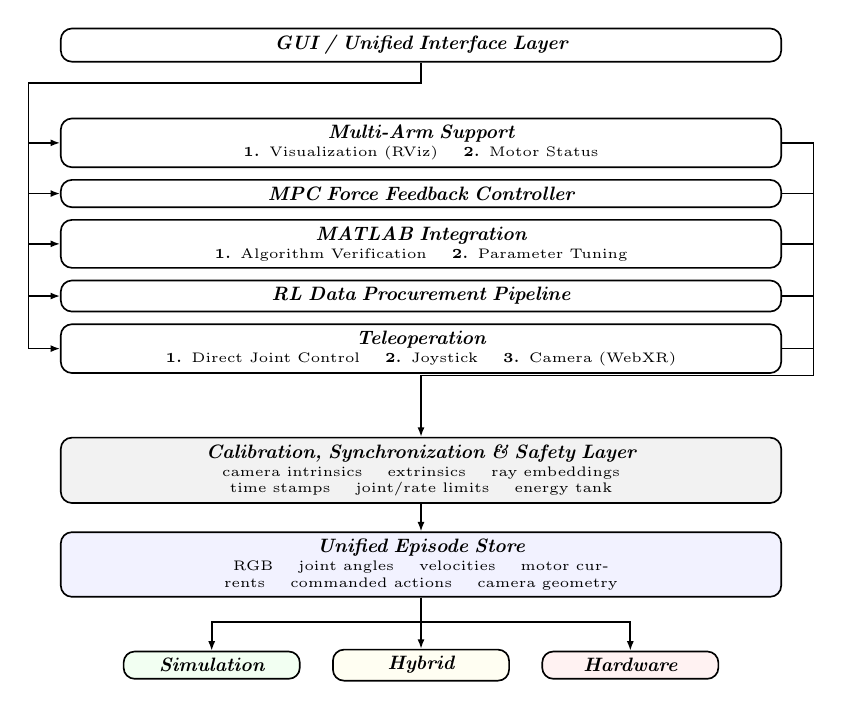
\begin{tikzpicture}[
    every node/.style={font=\tiny},
    block/.style={
        rectangle, draw, semithick, rounded corners,
        align=center, fill=white, inner sep=2.5pt
    },
    hdr/.style={font=\scriptsize\itshape\bfseries},
    arrow/.style={semithick, -{Latex[scale=0.6]}}
]

% ---- Stage 2: five modules ----
\node[block, text width=0.74\columnwidth] (multiarm)
  {{\hdr Multi-Arm Support}\\[0.5pt]
   \textbf{1.} Visualization (RViz) \quad \textbf{2.} Motor Status};

\node[block, text width=0.74\columnwidth, below=0.14cm of multiarm] (mpc)
  {{\hdr MPC Force Feedback Controller}};

\node[block, text width=0.74\columnwidth, below=0.14cm of mpc] (matlab)
  {{\hdr MATLAB Integration}\\[0.5pt]
   \textbf{1.} Algorithm Verification \quad \textbf{2.} Parameter Tuning};

\node[block, text width=0.74\columnwidth, below=0.14cm of matlab] (rl)
  {{\hdr RL Data Procurement Pipeline}};

\node[block, text width=0.74\columnwidth, below=0.14cm of rl] (teleop)
  {{\hdr Teleoperation}\\[0.5pt]
   \textbf{1.} Direct Joint Control \quad \textbf{2.} Joystick \quad \textbf{3.} Camera (WebXR)};

% ---- Stage 1: GUI ----
\node[block, text width=0.74\columnwidth, above=0.7cm of multiarm] (gui)
  {{\hdr GUI / Unified Interface Layer}};

% ---- Left bus: GUI -> all modules ----
\coordinate (lbus) at ([xshift=-0.4cm]multiarm.west);
\draw[semithick] (gui.south) -- ++(0,-0.26) -| (multiarm.west -| lbus);
\draw[semithick] (multiarm.west -| lbus) -- (teleop.west -| lbus);
\draw[arrow] (multiarm.west -| lbus) -- (multiarm.west);
\draw[arrow] (mpc.west      -| lbus) -- (mpc.west);
\draw[arrow] (matlab.west   -| lbus) -- (matlab.west);
\draw[arrow] (rl.west       -| lbus) -- (rl.west);
\draw[arrow] (teleop.west   -| lbus) -- (teleop.west);

% ---- Stage 3: calibration / synchronization / safety ----
\node[block, fill=gray!10, text width=0.74\columnwidth, below=0.8cm of teleop] (cal)
  {{\hdr Calibration, Synchronization \& Safety Layer}\\[0.5pt]
   camera intrinsics \quad extrinsics \quad ray embeddings \quad time stamps \quad joint/rate limits \quad energy tank};

% ---- Right bus: all modules -> calibration ----
\coordinate (rbus)  at ([xshift=0.4cm]multiarm.east);
\coordinate (rbot)  at (teleop.east -| rbus);
\coordinate (rjoin) at ([yshift=-0.34cm]rbot);
\draw[semithick] (multiarm.east) -- (multiarm.east -| rbus);
\draw[semithick] (mpc.east)      -- (mpc.east      -| rbus);
\draw[semithick] (matlab.east)   -- (matlab.east   -| rbus);
\draw[semithick] (rl.east)       -- (rl.east       -| rbus);
\draw[semithick] (teleop.east)   -- (teleop.east   -| rbus);
\draw[semithick] (multiarm.east -| rbus) -- (rjoin);
\draw[arrow] (rjoin) -| (cal.north);

% ---- Stage 4: unified episode store ----
\node[block, fill=blue!5, text width=0.74\columnwidth, below=0.35cm of cal] (store)
  {{\hdr Unified Episode Store}\\[0.5pt]
   RGB \quad joint angles \quad velocities \quad motor currents \quad
   commanded actions \quad camera geometry};
\draw[arrow] (cal.south) -- (store.north);

% ---- Stage 5: execution modes ----
\node[block, fill=yellow!5, text width=0.17\columnwidth, below=0.65cm of store] (hybrid)
  {{\hdr Hybrid}};
\node[block, fill=green!5, text width=0.17\columnwidth, left=0.4cm of hybrid] (sim)
  {{\hdr Simulation}};
\node[block, fill=red!5, text width=0.17\columnwidth, right=0.4cm of hybrid] (hw)
  {{\hdr Hardware}};

\draw[arrow] (store.south) -- ++(0,-0.31) -| (sim.north);
\draw[arrow] (store.south) -- ++(0,-0.31) -| (hw.north);
\draw[arrow] (store.south) -- (hybrid.north);

\end{tikzpicture}
\caption{High-level architecture of MERLIN. The unified interface drives five experimental modules, all routed through a shared calibration, synchronization, and safety layer into a unified episode store consumed by three execution modes.}
\label{fig:architecture}
\end{figure}

% \vspace{-0.25cm}
\subsection{Teleoperation Module}

To support a wide spectrum of teleoperation needs, the testbed features a multi-tiered teleoperation module. The architecture is designed to decouple the user input interface from the low-level hardware, funneling all commands through a common middleware. This results in the following three tiers of teleoperation, direct joint-level control using both, an MPC based bilateral teleoperation and a joint publishing UI built into the test bench, Spatial Teleoperation using WebXR and Joystick-based Cartesian control.

% This modular design is inspired by OPEN TEACH \cite{iyer2024openteach}, which showed that separating the input device from the robot makes it easier to use the same teleoperation system with different robotic platforms. It has been demonstrated by GELLO \cite{wu2023gello} that, kinematically matched arm manipulator master devices can provide better teleoperation performance than VR controllers or 3D mice for complex bimanual manipulation tasks.
%This modular approach follows the design philosophy of OPEN TEACH \cite{iyer2024openteach}, which demonstrated that decoupling input modality from robot morphology enables plug-and-play teleoperation across diverse platforms. Similarly, GELLO \cite{wu2023gello} showed that kinematically-matched,  teleoperation devices can outperform VR controllers and spacemouse interfaces for complex bimanual tasks.

\subsection{Multi-Arm Interoperability}
% \vspace{-0.25cm}
The platform enables the selection and control of multiple heterogeneous robotic arms within a unified software stack, eliminating the need for separate middleware configurations per robot. This is achieved through a modular abstraction layer that provides plug-and-play integration for any manipulator equipped with standard ROS2 interfaces, standardizing control protocols across different manufacturers. This capability is essential for bimanual manipulation research, where coordinated control of two or more arms is required, and for scalable data collection workflows where multiple robots operate simultaneously \cite{dass2023pato, unibidex}.

% \subsection{Control Parameter Tuning}
% The testbed provides an integrated environment for systematic controller tuning. Researchers can define parameter sweeps over controller configurations, including PID gains, MPC prediction horizons, and impedance parameters, and execute them without manual intervention. This feature supports automated optimization pipelines where the parameter space is explored efficiently, and results are logged alongside the corresponding episode data for later analysis.

% The importance of careful parameter tuning is well established in the robotics literature. Iqbal \cite{iqbal2019matlab} demonstrated that H-infinity and MPC controllers for robotic manipulators require systematic fine-tuning in simulation before deployment. Arm-Bench extends this workflow by coupling MATLAB-based optimization with the unified episode store, so that every parameter configuration is associated with its complete execution trace.

\subsection{RL Data Collection and Training}
MERLIN logs synchronized encoder, camera, and operator streams in HDF5, so one format covers teleoperated demonstration collection through policy training.

The pipeline follows three principles. First, data quality depends on synchronization, delay handling, and action representation: all streams are time-aligned and every observation and action is stored with a raw timestamp. Second, scalable collection can use assisted teleoperation: the teleoperation module is designed to accept assistive policies that automate repetitive subtasks without changing the logging (not yet implemented). Third, the same control interface can host active strategies such as goal-conditioned exploration, so collection, logging, and evaluation share one platform.

Images are stored with camera geometry: intrinsics \(\bm{K}\) (focal length, principal point, distortion); extrinsics \(\bm{T}_{\text{world}}^{\text{cam}}\); per-pixel ray embeddings from \(\bm{K}\) and \(\bm{T}_{\text{world}}^{\text{cam}}\); and per-frame pose metadata. One dataset then trains (1)~RGB-only policies, (2)~RGB + geometry policies, and (3)~camera-frame action policies, with end-effector actions in the camera frame so geometry stays consistent across embodiments and viewpoints. The same logs therefore support geometry-aware versus geometry-agnostic comparison.

% \subsection{RL Data Collection and Training}
% The platform provides an end-to-end RL data pipeline that logs synchronized streams from motor encoders, cameras, and operator inputs in HDF5, so the same format can be used from teleoperated demonstration collection through policy training.

% The pipeline follows three principles from recent work. First, data quality depends on synchronization, delay handling, and action representation. MERLIN time-aligns all sensor streams and stores raw timestamps for every observation and action. Second, scalable collection benefits from assisted teleoperation: the teleoperation module accepts assistive policies as pluggable components, so repetitive subtasks can be automated without changing the logging stack. Third, the same control interface supports active collection strategies, including goal-conditioned exploration, so researchers can collect, log, and evaluate data under one platform.

% Unlike platforms that treat images as unstructured buffers, MERLIN stores camera geometry with each observation: the intrinsic matrix $\bm{K}$ (focal length, principal point, distortion); extrinsics $\bm{T}_{\text{world}}^{\text{cam}}$; per-pixel ray embeddings derived from $\bm{K}$ and $\bm{T}_{\text{world}}^{\text{cam}}$; and per-frame camera-pose metadata. The same logged dataset then supports three training modes: (1)~RGB-only policies; (2)~RGB + geometry policies that add intrinsics, extrinsics, and ray embeddings; and (3)~camera-frame action policies, with end-effector actions expressed in the camera frame so geometric semantics stay consistent across embodiments and camera placements. This lets the same data be used to compare geometry-aware and geometry-agnostic policies.

% \subsection{RL Data Collection and Training}
% % \vspace{-0.25cm}
% The platform provides a complete data acquisition pipeline for reinforcement learning, capturing synchronized streams from motor encoders, camera feeds, and operator inputs. The unified data format (HDF5) is directly compatible with standard RL training frameworks, enabling seamless transition from teleoperated demonstration collection to policy learning.

% The data collection pipeline is designed around three principles drawn from the recent literature. 
% % First, the RL setup study by \cite{mahmood2018senseact} showed that data quality depends critically on synchronization, delay management, and action representation. 
% MERLIN addresses data quality deterioration  by enforcing strict time-alignment across all sensor streams and logging raw timestamps for every observation and action. Second, scalable data collection benefits from assisted teleoperation. 
% % PATO \cite{dass2023pato} demonstrated that automating repetitive subtasks through a hierarchical assistive policy reduces operator burden and enables single-operator, multi-robot data collection. 
% MERLIN teleoperation module is designed to integrate such assistive policies as pluggable components. Third, the platform supports active data collection strategies. Endrawis et al. \cite{endrawis2021efficient} showed that goal-conditioned active exploration produces more diverse datasets than random collection, and MERLIN modular control interface allows researchers to implement and evaluate such strategies within the same platform used for data logging.

% Unlike conventional RL platforms that treat camera images as unstructured observation buffers, MERLIN explicitly captures camera geometry as part of the observation space. For each camera, the platform stores Camera intrinsics matrix $\bm{K}$ (focal length, principal point, distortion coefficients); Camera extrinsics $\bm{T}_{\text{world}}^{\text{cam}}$ (rotation and translation from world frame to camera frame); Per-pixel ray embeddings computed from $\bm{K}$ and $\bm{T}_{\text{world}}^{\text{cam}}$ ; Camera pose metadata for each captured frame

% % This design is directly informed by the camera-conditioning work of Jiang et al. \cite{jiang2025kyknow}, who showed that providing camera intrinsics and extrinsics, together with Pl\"{u}cker ray embeddings, enables policies to generalize across viewpoints without exploiting background shortcuts. It also aligns with the multi-view representation learning approach of Maniwhere \cite{wei2024maniwhere}, which uses spatial transformer networks and curriculum randomization to achieve viewpoint-robust visual RL.

% The geometry-aware pipeline supports three training modalities: RGB-only policies: standard visual observations without explicit geometry. 2) RGB + geometry policies: visual observations augmented with camera intrinsics, extrinsics, and ray embeddings. 3) Camera-frame action policies: end-effector actions expressed in the camera coordinate frame, enabling consistent geometric semantics across different robot embodiments and camera placements.
% This multi-modal design ensures that the same logged dataset can be used to train and evaluate policies under different observation and action representations, supporting systematic comparison of geometry-aware versus geometry-agnostic approaches.

\subsection{Bimanual Bilateral Teleoperation}
% \vspace{-0.25cm}

% One of the major challenges on the majority of research arms, including the interbotix XS arms is the absence of dedicated force-torque sensors. To tackle this, the system implements a four-channel bilateral teleoperation architecture with force feedback without any explicit force sensor, supporting Master impedance and Slave admittance control modalities (MISA)\cite{MPCcontroller, impedance_origin}. Real-time trajectory tracking and integrated force sensing are governed by an MPC controller, implemented on a master-slave teleoperation setup using Interbotix ReactorX 200 and ViperX 300S arms, respectively, with the forearm-roll joint kinematically locked as shown in Fig. \ref{fig:setup}.

One of the major challenges on most research arms, including the Interbotix XS series, is the lack of a dedicated force-torque sensor. External force is therefore estimated from motor current, as in the sensorless approaches of Murakami et al.\ \cite{murakami1993} and De~Luca and Mattone \cite{delucamattone2003}. The platform implements force-reflecting bilateral teleoperation with this estimate, using master-impedance / slave-admittance (MISA) control \cite{MPCcontroller,impedance_origin}. Real-time tracking is handled by a constrained MPC on a master--slave pair (ReactorX 200 / ViperX 300S) with the forearm-roll joint locked, which leaves $n=5$ active joints, as in Fig.~\ref{fig:setup}.

\begin{figure}[thbp]
    \centering
    \includegraphics[width=0.5\linewidth]{images/2026-07-11-234643.jpg}
    \caption{Bilateral Teleoperation Setup: master1, master2, slave1 and slave2 (From Top left, left to right)}
    \label{fig:setup}
\end{figure}

\subsubsection{Notation:}
A first-order IIR filter with coefficient $\alpha$ is written
$\mathcal{F}_\alpha\{x\}[k]=\alpha\,x[k]+(1-\alpha)\,\mathcal{F}_\alpha\{x\}[k-1]$,
with $\alpha_v=0.3$ where it is used. Saturation and dead-zone act elementwise:
$\mathrm{sat}_{a}(x)=\mathrm{clip}(x,-a,a)$ and
$\mathrm{dz}_{\delta}(x)=\mathrm{sign}(x)\max(|x|-\delta,0)$.
The weighted norm is $\|x\|_{W}^{2}=x^{\top}Wx$.

\subsubsection{State, Force, and Torque Estimation:}
Motors run in current-based mode with torque enabled. The motor torque follows from the measured current $I$ (in mA, as published by the Interbotix driver) as $\tau_m=n_\mu\odot k_t\odot10^{-3}I$, where $k_t$ is the torque constant and $n_\mu$ the number of motors driving a joint (two for the RX200 shoulder and for the VX300S shoulder and elbow). With the rigid-body model
$M(q)\ddot q+C(q,\dot q)\dot q+G(q)=\tau_m+\tau_{ext}$, the external torque $\tau_{ext}$ (contact, operator, unmodelled friction) is the dynamics residual. Neglecting $M\ddot q$ gives the static residual
\begin{equation}
\hat\tau^{\mathrm{static}}=G(q)+C(q,\dot q)\dot q-\tau_m=\tau_{ext}-M(q)\ddot q,
\end{equation}
which is exact only at rest: during motion $-M\ddot q$ appears as a false contact torque (in simulation 0.25, 0.48, and 1.08\,N\,m rms at one, two, and three times the nominal speed). We therefore estimate $\tau_{ext}$ with the generalised-momentum observer \cite{delucamattone2003}. With $p=M(q)\dot q$ and gain $K_O=\mathrm{diag}(k_i)$,
\begin{equation}
r=K_O\Big(p-p(0)-\int_0^t\big(\tau_m+C^{\top}\dot q-G+r\big)\,ds\Big),
\qquad \dot r=K_O(\tau_{ext}-r),
\label{eq:observer}
\end{equation}
so $r$ is $\tau_{ext}$ low-pass filtered at $k_i$\,rad/s and no acceleration is needed. With $K_O=15$\,rad/s at $\Delta t=0.02$\,s the sampled observer is a first-order filter with coefficient $K_O\Delta t=0.3$ (stable and monotone for $K_O\Delta t<1$). It is fed the unfiltered velocity and torque: the IIR-filtered velocity of the first implementation lags $p$ by about $47$\,ms and excited a master--slave limit cycle in simulation. The estimate inherits the errors of $k_t$ and of the link masses, so both must be calibrated with known weights on the real arms.

\subsubsection{Master Impedance Law:}
With the operator torque $\tau_h=J_m^{\top}F_h$,
\begin{equation}
M_m\ddot q_m+C_m\dot q_m+G_m=\tau_{m}+\tau_h,
\qquad
\tau_{m,cmd}=\hat G_m(q_m)-D_{md}\,\dot q_m+\gamma\,\tau_f .
\end{equation}
The commanded torque does not depend on the master's own measured current. (A law that subtracts the measured torque estimate from itself has a pole at $z=1$ and integrates any constant bias, such as a gravity-model error, until the torque clamp.) With $\tau_f=0$ the master is output-strictly passive from $\tau_h$ to $\dot q_m$; $\tau_f$ is the force-feedback torque below and $\gamma\in[0,1]$ the energy-tank gate.

\subsubsection{Slave Admittance Law:}
\begin{equation}
\begin{aligned}
M_d\ddot q_e+D_d\dot q_e+K_dq_e&=\mathrm{dz}_{\delta}\big(\hat\tau_{ext,s}\big),\\
q_{s,ref}&=Sq_m+o+q_e,
\end{aligned}
\end{equation}
with design parameters $M_d,D_d,K_d>0$ per joint (critically damped, natural frequency about $10$\,rad/s), a per-joint soft dead-zone $\delta$, and the master-to-slave scaling $S,o$. The admittance is discretised exactly for a zero-order hold (augmented matrix exponential, Van~Loan \cite{vanloan1978}). Explicit Euler is unusable here: with the physical inertia as $M_d$ of the first implementation, the wrist-rotate eigenvalue $|1+\lambda\Delta t|=9.45>1$.

\subsubsection{Force and Position Feedback:}
Three signals cross the link: the master position (to the slave), and the estimated slave contact torque and the slave position (to the master). The slave wrench is estimated by damped least squares, $\hat F_s=J_s(J_s^{\top}J_s+\lambda^2I)^{-1}\mathrm{dz}_{\delta}(\hat\tau_{ext,s})$, and mapped to the master through its Jacobian, which corrects the over-rendering of about $1.4\times$ that one-to-one joint-torque reflection gives between arms of different reach:
\begin{equation}
\tau_f=k_{of}\,J_m^{\top}S_f\,\hat F_s-k_{om}K_{md}\,(Sq_m+o-q_s).
\end{equation}
The gate $\gamma$ comes from an energy tank with state $T\in[T_{\min},T_{\max}]$: the energy delivered to the operator, $\sum\Delta t\,\gamma\,\tau_f^{\top}\dot q_m$, cannot exceed the tank's initial energy above $T_{\min}$ plus the energy the master dissipates. This bounds the \emph{master-side} power only; it does not provide stability under communication delay \cite{anderson1989,hannaford2002}.

\subsubsection{Slave Tracking:}
The VX300S is commanded in position, so the MPC chooses position commands $u$, not torques. Each joint is modelled by the identified position loop of the Dynamixel servo, $\ddot q_i=\omega_i^2(u_i-q_i)-2\zeta_i\omega_i\dot q_i+c_i$, discretised exactly, with an output-disturbance estimate $\hat d$ (a low-pass filter of the model error) that makes the controller offset-free \cite{pannocchia2003}. With predictions $\hat q_k,\hat v_k$ over $N=10$ steps ($200$\,ms), the reference preview $r_k=q_{s,ref}+k\Delta t\,S\dot q_m$, and the previous command $u_{-1}$,
\begin{equation}
\begin{aligned}
\min_{u_{0:N-1}}\;&\sum_{k=1}^{N}w_k\big(\hat q_k-r_k\big)^{2}+R\sum_{k=0}^{N-1}\big(u_k-u_{k-1}\big)^{2}\\
\text{s.t.}\;&q_{\min}\le u_k\le q_{\max},\quad|u_k-u_{k-1}|\le\Delta u_{\max},\quad|\hat v_k|\le\dot q_{\max},
\end{aligned}
\label{eq:slave_mpc}
\end{equation}
with $w_k=Q$ for $k<N$ and $w_N=P$. The problem is a strictly convex quadratic program per joint; it is solved by ADMM \cite{stellato2020osqp} with a factorisation computed once, in about $1$\,ms per tick for five joints, and $u_0^{\star}$ is applied. The position-loop parameters $\omega_i,\zeta_i$ were identified on the simulated arm; on the real arm they must be identified from a step test before the MPC is used.

% \subsubsection{State estimation}
% \begin{itemize}
%     \item Joint Velocity is estimated via backward difference with first order IIR smoothing
%     \begin{equation}
%         \dot{q}_{raw}[k] = \frac{q[k]-q[k-1]}{\Delta t}, \qquad \\[5pt]
        
% \dot{q}[k] = \alpha_v\,\dot{q}_{raw}[k] + (1-\alpha_v)\,\dot{q}[k-1], \quad \alpha_v = 0.3
%     \end{equation}
% \end{itemize}
% \subsubsection{Force and Torque Estimation}
% The motors are all set to Current-based operating mode with the Torque enabled.
% \begin{itemize}
%     \item Torque Estimation from Motor Current

% Motor torque is estimated using:
% \begin{equation}
%     \tau_{raw}[k] = k_t \odot I[k], \qquad 
    
% \tau_{motor}[k] = \alpha_v\,\tau_{raw}[k] + (1-\alpha_v)\,\tau_{motor}[k-1]
% \end{equation}
% where:
% \begin{itemize}
%     \item $K_t$ is the motor torque constant
%     \item $\bm{I}_{\text{measured}}$ is the motor current
% \end{itemize}

% \item External Torque is estimated as a residual, with the inertial term omitted
% \begin{equation}
% \hat{\tau}_{ext} = \tau_{motor} - \big(C(q,\dot q) + G(q)\big)
% \end{equation}
% \end{itemize}

% \subsubsection{Master Dynamics}

% \begin{equation}
%     \begin{gathered}
%         M_m \ddot{q}_m + C_m(\dot{q}_m, q_m) + G_m = \tau_m + J_m^{T} F_h \\
%         \tau_{m,cmd} = G_m - D_{md}\,\dot q_m + \tau_{ext,m}^{tot} \\
%     \end{gathered}
% \end{equation}

% \subsubsection{Slave Admittance Law}

% \begin{equation}
%     \begin{gathered}
%         \tau_{refl} = k_{of}\,\hat\tau_{ext,m}, \qquad \\[5pt]

%         \tau_{adm} = \mathrm{clip}\big(\hat\tau_{ext,s} - \tau_{refl},\ -\tau_{max}^{motor},\ \tau_{max}^{motor}\big)
%         \\[5pt]
%         M_{s}\,\ddot q_e + D_{s}\,\dot q_e + K_{s}\,q_e = \tau_{adm}
%         \\[5pt]
%         \ddot q_e = (M_{sd} + \varepsilon I)^{-1}\big(\tau_{adm} - D_{sd}\dot q_e - K_{sd} q_e\big), \quad \varepsilon = 10^{-4}
%         \\[5pt]
%         q_{s,ref} = q_m + q_e
%     \end{gathered}
% \end{equation}

% ==========================================================================
% \subsubsection{State estimation:}Joint Velocity is estimated via backward difference with first order IIR smoothing
% % \begin{equation}
% %     \begin{gathered}
% %         \dot{q}_{raw}[k] = \frac{q[k]-q[k-1]}{\Delta t}, \\
% %         \dot{q}[k] = \alpha_v\,\dot{q}_{raw}[k] + (1-\alpha_v)\,\dot{q}[k-1],\alpha_v = 0.3
% %     \end{gathered}
% % \end{equation}

% \begin{equation}
% \begin{aligned}
%     \dot{q}_{raw}[k] &= \frac{q[k]-q[k-1]}{\Delta t}, \\
%     \dot{q}[k] &= \alpha_v\,\dot{q}_{raw}[k]
%                + (1-\alpha_v)\,\dot{q}[k-1], \\
%     \alpha_v &= 0.3.
% \end{aligned}
% \end{equation}

% \subsubsection{Force and Torque Estimation:}The motors are all set to Current-based operating mode with the Torque enabled.

% Torque Estimation from Motor Current
% Motor torque is estimated using:
% \begin{equation}
% \begin{aligned}
%     \tau_{raw}[k] &= k_t \odot I[k], \\
%     \tau_{motor}[k] &= \alpha_v\,\tau_{raw}[k]
%     + (1-\alpha_v)\,\tau_{motor}[k-1],
% \end{aligned}
% \end{equation}
% \noindent
% where $k_t$ denotes the motor torque constant, $I[k]$ is the measured motor current, and $\alpha_v$ is the IIR filter coefficient.
% % \begin{equation}
% %     \begin{gathered}
% %         \tau_{raw}[k] = k_t \odot I[k], \\[5pt]
% %         \tau_{motor}[k] = \alpha_v\,\tau_{raw}[k] + (1-\alpha_v)\,\tau_{motor}[k-1]
% %     \end{gathered}
% % \end{equation}

% % \begin{itemize}
% %     \item $k_t$ is the motor torque constant
% %     \item $I[k]$ is the measured motor current
% % \end{itemize}

% % \begin{equation}
% % \begin{aligned}
% %     \tau_{raw}[k] &= k_t \odot I[k], \\
% %     \tau_{motor}[k] &= \alpha_v\,\tau_{raw}[k]
% %     + (1-\alpha_v)\,\tau_{motor}[k-1],
% % \end{aligned}
% % \quad
% % \begin{aligned}[t]
% % \text{where } \;
% % k_t &:\ \text{motor torque constant},\\
% % I[k] &:\ \text{measured motor current},\\
% % \alpha_v &:\ \text{IIR filter coefficient}.
% % \end{aligned}
% % \end{equation}


% External Torque is estimated as a residual
% \begin{equation}
%     \begin{aligned}
%         \hat{\tau}_{ext} &= \tau_{motor} - \big(C(q,\dot q) + G(q)\big)
%     \end{aligned}
% \end{equation}

% \subsubsection{Master Impedance Law :}
% \begin{equation}
%     \begin{aligned}
%         M_m \ddot{q}_m + C_m(\dot{q}_m, q_m) + G_m &= \tau_m + J_m^{T} F_h \\
%         \tau_{m,cmd} &= G_m - D_{md}\,\dot q_m + \tau_{ext,m}^{tot}
%     \end{aligned}
% \end{equation}

% \subsubsection{Slave Admittance Law:}

% % \begin{equation}
% %     \begin{aligned}
% %         \tau_{refl} &= k_{of}\,\hat\tau_{ext,m}, \\[5pt]
% %         \tau_{adm} &= \mathrm{clip}\big(\hat\tau_{ext,s} -\tau_{refl}, -\tau_{max}^{motor},\ \tau_{max}^{motor}\big) \\[5pt]
% %         M_{s}\,\ddot q_e + D_{s}\,\dot q_e + K_{s}\,q_e &= \tau_{adm} \\[5pt]
% %         \ddot q_e &= (M_{sd} + \varepsilon I)^{-1}\big(\tau_{adm} - D_{sd}\dot q_e \\- K_{sd} q_e\big), \quad\varepsilon &= 10^{-4} \\[5pt]
% %         q_{s,ref} &= q_m + q_e
% %     \end{aligned}
% % \end{equation}

% % \begin{equation}
% % \begin{aligned}
% %     \tau_{refl} &= k_{of}\,\hat{\tau}_{ext,m}, \\
% %     \tau_{adm} &= \mathrm{clip}
% %     \left(
% %         \hat{\tau}_{ext,s}-\tau_{refl},
% %         -\tau_{max}^{motor},
% %         \tau_{max}^{motor}
% %     \right), \\
% %     M_s\ddot q_e + D_s\dot q_e + K_s q_e
% %     &= \tau_{adm}, \\
% %     \ddot q_e
% %     &= (M_{sd}+\varepsilon I)^{-1}
% %     \Big(
% %         \tau_{adm}
% %         - D_{sd}\dot q_e
% %         - K_{sd}q_e
% %     \Big), \\
% %     q_{s,ref} &= q_m + q_e.
% % \end{aligned}
% % \end{equation}

% % \noindent
% % where $\varepsilon = 10^{-4}$ is a regularization constant.
% % \begin{equation}
% % \begin{aligned}
% %     \tau_{refl} &= k_{of}\,\hat{\tau}_{ext,m}, \\[3pt]
% %      \tau_{adm} &= \mathrm{clip}
% %     (
% %         \hat{\tau}_{ext,s}-\tau_{refl},\\
% %         &\qquad-\tau_{max}^{motor},
% %         \tau_{max}^{motor}
% %     ), \\[3pt]
% %     M_s\ddot q_e + D_s\dot q_e + K_s q_e
% %     &= \tau_{adm}, \\[3pt]
% %     \hspace{-3.5cm} \ddot q_e
% %     &= (M_{sd}+\varepsilon I)^{-1}
% %     \Big(
% %         \tau_{adm}
% %         - D_{sd}\dot q_e \\
% %     &\qquad
% %         - K_{sd}q_e
% %     \Big), \qquad
% %     \varepsilon = 10^{-4}, \\[3pt]
% %     q_{s,ref} &= q_m + q_e.
% % \end{aligned}
% % \end{equation}

% \begin{equation}
% \begin{aligned}
%     & \tau_{refl} = k_{of}\,\hat{\tau}_{ext,m}, \\[3pt]
%     & \tau_{adm} = \mathrm{clip}
%     \begin{aligned}[t]
%         \Big( &\hat{\tau}_{ext,s}-\tau_{refl},
%               &-\tau_{max}^{motor}, \tau_{max}^{motor} \Big)
%     \end{aligned}, \\[3pt]
%     & M_s\ddot q_e + D_s\dot q_e + K_s q_e = \tau_{adm}, \\[3pt]
%     & \ddot q_e = (M_{sd}+\varepsilon I)^{-1}
%     \begin{aligned}[t]
%         \Big( &\tau_{adm} - D_{sd}\dot q_e & \hspace{-0.2cm}- K_{sd}q_e \Big)
%     \end{aligned},  \varepsilon = 10^{-4}, \\[3pt]
%     & q_{s,ref} = q_m + q_e.
% \end{aligned}
% \end{equation}

% \subsubsection{Four Channel feedback:}A soft dead-zone is applied to the slave's contact-force estimate before it is rendered to the operator, per joint threshold $\delta_i$
% \begin{equation}
%     \begin{aligned}
%         \tilde\tau_{ext,s,i} &= \mathrm{sign}(\hat\tau_{ext,s,i})\,\max\!\big(|\hat\tau_{ext,s,i}| - \delta_i,\ 0\big) \\
%         \tau_{f} &= -k_{of}\,\tilde\tau_{ext,s}, \qquad \\
%         \tau_{p} &= -k_{om}\,K_{md}(q_m - q_s) \\
%         \tau_{ext,m}^{tot} &= \hat\tau_{ext,m} + \tau_f + \tau_p
%     \end{aligned}
% \end{equation}
% The four-channel architecture exchanges position, velocity, force, and auxiliary signals between master and slave.
% % , achieving transparency under ideal conditions while maintaining passivity through energy tank monitoring \cite{article_minetal}.

% \subsubsection{Slave Tracking:}The MPC Algorithm minimizes over the horizon, $N=3$ at $\Delta t = 0.02s$
% % \begin{equation}
% %     \begin{gathered}
% %         \min \sum_{k=0}^{N-1}\Big[(q_k - q_{s,ref})^\top Q_s (q_k - q_{s,ref}) + \\ \tau_k^\top R_s \tau_k + \Delta\tau_k^\top S_s \Delta\tau_k\Big] + (q_N - q_{s,ref})^\top P_s (q_N - q_{s,ref}) \\
% %         \text{s.t.}\quad q_{min}\le q_k \le q_{max},\ \ \dot q_{min}\le \dot q_k \le \dot q_{max},\ \ \tau_{min}\le \tau_k \le \tau_{max}
% %     \end{gathered}
% % \end{equation}

% \begin{equation}
% \begin{aligned}
%     \min_{\tau_{0:N-1}} \quad &
% \sum_{k=0}^{N-1}
% \Big[
% (q_k-q_{s,\mathrm{ref}})^{\top}Q_s(q_k-q_{s,\mathrm{ref}})
% +\tau_k^{\top}R_s\tau_k \\
% &\hspace{2.8cm}
% +\Delta\tau_k^{\top}S_s\Delta\tau_k
% \Big] \\
% &+(q_N-q_{s,\mathrm{ref}})^{\top}P_s(q_N-q_{s,\mathrm{ref}})
% \\[0.5em]
% \text{s.t.}\quad
% &q_{\min}\le q_k \le q_{\max}, \\
% &\dot{q}_{\min}\le \dot{q}_k \le \dot{q}_{\max}, \\
% &\tau_{\min}\le \tau_k \le \tau_{\max},
% \end{aligned}
% \label{eq:slave_mpc}
% \end{equation}
% ==========================================================================


\subsection{Integrated Control Algorithm Development and Parameter Tuning}
Unlike platforms that treat control design as an external process, MERLIN includes an in-UI development environment with syntax checking, real-time compilation, and in-application execution, so algorithms can be written, tested, and iterated without leaving the testbed. Controllers can also be loaded from parameter files for systematic gain sweeps and automated tuning, with MATLAB used for optimization workflows that require no manual intervention. Tunable parameters are declared in the control script itself with an annotation comment, e.g.\ \texttt{\% @param min=0 max=50 desc="proportional gain"} above \texttt{Kp = 8;}; the GUI reads the declaration to create the parameter field, its bounds, and the search range of the tuner, so the script is the single source of truth.

MATLAB integration is bidirectional: algorithms from MATLAB/Simulink can be verified on the MERLIN simulation backend before hardware deployment, and real execution traces can be exported for post-hoc analysis and retuning. Every parameter set is stored with its full execution trace in the unified episode store.

\subsection{Hybrid Simulation Operations}
Control algorithms can be validated in simulation before hardware deployment, or run concurrently with the real robot for sim-to-real studies. This is useful for safe RL exploration and for tests that would be costly or unsafe on hardware alone.

Hybrid mode uses a shared episode format: simulated observations, joint states, and actions during sim episodes; physical counterparts during hardware episodes. In concurrent hybrid operation, a learned policy can run in simulation while physical sensor data are recorded, so simulated and real behavior can be compared on the same timestep.

By combining these capabilities in one extensible platform, MERLIN removes the need for separate stacks for teleoperation, control development, data collection, and simulation.

% \subsection{Integrated Control Algorithm Development and \\Parameter Tuning}
% % \vspace{-0.25cm}
% Unlike existing platforms that treat control design as an external process, the testbed incorporates an integrated development environment with syntax checking, real-time code compilation, and in-application execution. Researchers can write, test, and iterate custom control algorithms directly within the UI, dramatically reducing the development cycle. The system supports loading control configurations from parameter files, enabling systematic sweeps over controller configurations to identify optimal controller gains, with MATLAB integration for parameter tuning and systematic optimization workflows. This feature supports automated tuning pipelines where parameter space exploration can be performed without manual intervention.

% The MATLAB integration follows a bidirectional design pattern. Control algorithms developed in MATLAB or Simulink can be verified against the MERLIN simulation backend before deployment on hardware, and real-world execution data can be exported to MATLAB for post-hoc analysis and parameter optimization. 
% % \textbf{Trivia again?}
% % This workflow is consistent with the simulation-to-reality paradigm demonstrated by Chaos et al. \cite{chaos2013virtual} and Cen et al. \cite{cen2025digitaltwin}, where MATLAB-based analysis complements real-world experimentation.
% % The importance of careful parameter tuning is well established in the robotics literature. Iqbal \cite{iqbal2019matlab} demonstrated that H-infinity and MPC controllers for robotic manipulators require systematic fine-tuning in simulation before deployment. 

% MERLIN extends this workflow by coupling MATLAB-based optimization with the unified episode store, so that every parameter configuration is associated with its complete execution trace.
% % where MATLAB-based analysis complements real-world experimentation.

% \subsection{Hybrid Simulation Operations}
% % \vspace{-0.25cm}
% The testbed supports hybrid workflows where control algorithms can be validated in simulation before deployment on physical hardware, or where simulation execution can operate concurrently for sim-to-real transfer studies. This capability is particularly valuable for safe exploration in RL and for testing control algorithms under conditions that would be expensive or dangerous on real hardware alone.

% The hybrid mode operates through a shared episode: the same data format captures simulated observations, simulated joint states, and simulated actions during simulation episodes, and physical observations, physical joint states, and physical actions during hardware episodes. When operating in hybrid mode, the platform can run a learned policy in simulation while simultaneously recording physical sensor data from the real robot, enabling direct comparison of simulated and real-world behavior within the same timestep record. 
% % This design is consistent with the sim-to-real transfer paradigm demonstrated by Zhu et al. \cite{zhu2018visuomotor}, who achieved zero-shot transfer by training with visual and dynamics randomization in simulation, and by Wei et al. \cite{wei2024maniwhere}, who used curriculum-based domain randomization to bridge the sim-to-real gap.

% % \subsection{Custom Control File Loading}


% By unifying these capabilities within a single, extensible platform, MERLIN addresses the fragmentation that currently forces researchers to maintain separate systems for teleoperation, control development, data collection, and simulation.

% \section{Experiments and Evaluation}
% The trajectory tracking performance of the proposed control testbed was evaluated by collecting $7,691$ synchronised Samples across a series of bilateral teleoperation tasks. For each sample, the desired joint angles of the RX-200 Arms commanded by the operator was recorded alongside the actual joint positions  executed by the VX-300s Arms, enabling frame by frame computation. The Gripper joint was linearly interpolated owing to the difference in dimensions of the 2 Arms.

% \begin{table}[h]
% \centering
% \caption{Joint Tracking Performance Metrics}
% \label{tab:tracking_metrics}
% \begin{tabular}{lccccc}
% \hline
% \textbf{Joint} & \textbf{RMSE} & \textbf{MAE} & \textbf{Max Error} & \textbf{P95 Error} & \textbf{Tracking Score} \\
% \hline
% Joint 0 & 0.2250 & 0.1355 & 1.2164 & 0.5239 & 0.8346 \\
% Joint 1 & 0.2715 & 0.1800 & 1.0569 & 0.6420 & 0.8480 \\
% Joint 2 & 0.3609 & 0.2492 & 1.3315 & 0.7961 & 0.7958 \\
% Joint 3 & 0.3152 & 0.1954 & 1.5555 & 0.7102 & 0.7602 \\
% Joint 4 & 0.5366 & 0.3736 & 1.4251 & 1.0301 & 0.3545 \\
% \hline
% \textbf{Overall} & \textbf{0.3418} & \textbf{0.2267} & \textbf{1.5555} & \textbf{0.7405} & \textbf{0.7186} \\
% \hline
% \end{tabular}
% \end{table}
% \vspace{-0.25cm}
\section{Experiments and Evaluation}
% \vspace{-0.35cm}
To quantitatively assess the capability of the system in maintaining precise joint-space synchronization under a real-time control loop, trajectory tracking was performed during a series of bilateral teleoperation tasks, encompassing both free-space motions and tasks that involve continuous contact with the environment. Throughout these experiments, the target joint trajectories, commanded by the operator via the RX-200 master manipulator, were recorded in parallel with the executed joint positions from the VX-300s slave manipulators.

In order to ensure the synchronization of the joint states from the heterogeneous arms, both systems were sampled simultaneously at a control frequency of $50Hz$. Due to differences in the kinematic scaling and movement range between the master and slave grippers, gripper commands were linearly scaled in an effort to ensure the highest possible degree of fidelity, thus permitting frame-by-frame calculation of instantaneous tracking error in each degree of freedom.

Table~\ref{tab:tracking_metrics} presents a summary of the tracking performance over the dataset by reporting the root-mean-square error (RMSE), mean absolute error (MAE), and maximum absolute error of the tracking error in each joint.

\begin{table}[th]
\centering
\caption{Joint tracking on the real arms with the controller as submitted (initial implementation; the revised controller is evaluated in Section~\ref{sec:sim}).}
\label{tab:tracking_metrics}
\resizebox{\columnwidth}{!}{%
\begin{tabular}{lccc}
\hline
\textbf{Joint} & \textbf{RMSE (rad)} & \textbf{MAE (rad)} & \textbf{Max Error (rad)} \\
\hline
Waist & 0.2250 & 0.1355 & 1.2164 \\
Shoulder & 0.2715 & 0.1800 & 1.0569 \\
Elbow & 0.3609 & 0.2492 & 1.3315 \\
Wrist Angle & 0.3152 & 0.1954 & 1.5555 \\
Wrist Rotate & 0.5366 & 0.3736 & 1.4251 \\
\hline
\textbf{Overall} & \textbf{0.3583} & \textbf{0.2267} & \textbf{1.5555} \\
\hline
\end{tabular}%
}
\end{table}

\subsection{Tracking Performance and Controller Efficacy}
% \vspace{-0.25cm}
% As demonstrated in Table~\ref{tab:tracking_metrics}, tracking errors are consistently lower for proximal joints (Waist, Shoulder) than for distal joints (Wrist Rotate). This trend is as expected, since kinematics naturally lead to increasing errors as the manipulator's link count grows. The overall positioning tracking performance of the Model Predictive Control (MPC) controller used is graphically illustrated in Fig.~\ref{fig:tracking_plot}, which depicts a scatter plot of actual vs. Target joint positions.
% While the system maintains an impressive level of synchronized operation with minimal drift (Overall RMSE of $0.3418$ rad), small tracking delays occur during rapid changes in movement direction. Such delays are inherent to computationally expensive, constrained optimization controllers, where torques must be calculated over a predictive horizon within the fixed $20ms$ time frame of the $50Hz$ control loop. The forearm-roll joint was restricted to remain fixed in position to decrease the complexity of the optimization problem in the MPC solver and reduce computation time; this constraint was found to be effective in guaranteeing rapid convergence for high-dimensional state-space MPC problems within the specified $20ms$ budget on this low-cost hardware platform, thus enabling the operation of computationally intensive control strategies.
As shown in Table~\ref{tab:tracking_metrics}, the error is smallest at the waist and shoulder and largest at the wrist-rotate joint. We do not attribute this to error accumulating along the kinematic chain: each joint is controlled by its own loop, and in the simulation of the same code the ordering of the joints follows the amplitude and speed of the commanded motion (Table~\ref{tab:sim_joints}). Separating task and kinematic contributions on hardware remains to be done. Overall tracking is shown in Fig.~\ref{fig:tracking_plot} as a scatter of actual versus target joint positions.

The controller as submitted tracked with an overall RMSE of $0.3583$\,rad (pooled over joints; the mean of the per-joint RMSEs is $0.3418$\,rad). A post-submission analysis of the code identified the main cause. The reference passed through a smoothing step $q\leftarrow0.95\,q+0.05\,q_{ref}$ at $50$\,Hz, a first-order lag with a time constant of $0.39$\,s, and the MPC output that was sent to the slave was identically zero, because its position-increment variable did not enter the prediction model. The small delays at direction changes are therefore a property of that implementation, not inherent to constrained MPC. The forearm-roll joint was held fixed, leaving five active joints.

\begin{figure}[htbp]
\centering
\includegraphics[width=\linewidth]{images/tracking_plot.png}
\caption{Position tracking performance of the MPC controller during continuous teleoperation.}
\label{fig:tracking_plot}
\end{figure}

\subsection{Revised Controller in Simulation}
\label{sec:sim}
The revised controller of the preceding sections was evaluated in MuJoCo 3.17 with models of the RX200 and VX300S built from the URDFs the controller uses (Pinocchio 4.1 for the controller's dynamics). The plant differs from the controller's model on purpose: link masses and inertias $+8\%$, joint damping and Coulomb friction unknown to the controller, $4096$-count encoders, and motor current quantised at $2.69$\,mA with $5$\,mA noise. The slave's Dynamixel position loop is a PD law whose gains were chosen by us, so the identified $\omega_i,\zeta_i$ describe this simulated servo and must be re-identified on hardware. The task lasts $24$\,s: $12$\,s of free motion and $12$\,s of two pushes into a wall ($k=2000$\,N/m). The operator is a spring--damper pulling the master towards a sinusoidal trajectory. Each of $5$ seeds redraws the sensor noise and the operator's amplitudes ($\pm25\%$), frequencies ($\pm15\%$), and phases. All numbers of this subsection come from simulation and are not comparable in magnitude with Table~\ref{tab:tracking_metrics}. ``Original code$^\dagger$'' denotes the first implementation re-implemented in the same simulator, with the smoothing step and zero MPC output described above.

% generated by paper/make_tables.py -- do not edit by hand
\begin{table}[t]
\centering
\caption{Simulation (MuJoCo), 5 seeds, mean$\pm$std. Each seed redraws sensor noise and the operator trajectory. RMSE is pooled over the five joints. Lag is resolved at the 20\,ms control period. Force corr.: Pearson correlation of the force felt at the master and the true wall force.}
\label{tab:sim_multiseed}
\resizebox{\columnwidth}{!}{%
\begin{tabular}{lcccc}
\hline
\textbf{Controller} & \textbf{RMSE free (rad)} & \textbf{RMSE all (rad)} & \textbf{Lag (ms)} & \textbf{Force corr.} \\
\hline
Original code$^\dagger$ & 0.220$\pm$0.016 & 0.164$\pm$0.010 & 338$\pm$6 & $-$0.58$\pm$0.03 \\
Unilateral & 0.025$\pm$0.001 & 0.031$\pm$0.002 & 30$\pm$2 & $-$0.23$\pm$0.31 \\
Position--position & 0.024$\pm$0.001 & 0.027$\pm$0.001 & 30$\pm$2 & 0.41$\pm$0.24 \\
Position--force & 0.025$\pm$0.001 & 0.025$\pm$0.002 & 30$\pm$2 & 0.23$\pm$0.64 \\
Proposed, no MPC & 0.025$\pm$0.001 & 0.026$\pm$0.001 & 20$\pm$0 & 0.30$\pm$0.75 \\
\textbf{Proposed} & 0.007$\pm$0.001 & 0.016$\pm$0.005 & 0$\pm$0 & 0.48$\pm$0.34 \\
\hline
\end{tabular}%
}
\end{table}

\begin{table}[t]
\centering
\caption{Simulation counterpart of Table~\ref{tab:tracking_metrics}: per-joint tracking error over the whole task, mean of 5 seeds. Not comparable in magnitude with the hardware table (different operator, plant and controller).}
\label{tab:sim_joints}
\resizebox{\columnwidth}{!}{%
\begin{tabular}{lcccccc}
\hline
& \multicolumn{3}{c}{\textbf{Original code}$^\dagger$} & \multicolumn{3}{c}{\textbf{Proposed}} \\
\textbf{Joint} & RMSE & MAE & Max & RMSE & MAE & Max \\
\hline
Waist & 0.1705 & 0.1283 & 0.4830 & 0.0129 & 0.0042 & 0.1449 \\
Shoulder & 0.0925 & 0.0782 & 0.2385 & 0.0056 & 0.0032 & 0.0409 \\
Elbow & 0.0982 & 0.0704 & 0.2893 & 0.0144 & 0.0100 & 0.0692 \\
Wrist Angle & 0.1430 & 0.0991 & 0.3707 & 0.0193 & 0.0114 & 0.1427 \\
Wrist Rotate & 0.2537 & 0.1869 & 0.6272 & 0.0142 & 0.0049 & 0.1681 \\
\hline
\end{tabular}%
}
\end{table}

\begin{table}[t]
\centering
\caption{Torque mimicking in simulation: known forces act on the slave gripper while the operator holds the master still. Gain: least-squares ratio of felt force to $k_{of}F_{env}$ (1 = exact scaled reproduction).}
\label{tab:sim_mimic}
\begin{tabular}{lccccc}
\hline
\textbf{Controller} & RMSE (N) & corr.\ $x$ & corr.\ $z$ & gain $x$ & gain $z$ \\
\hline
Original code$^\dagger$ & 3.41 & 0.53 & 0.25 & $-$0.12 & 1.13 \\
Position--force & 0.34 & 0.96 & 0.98 & 0.94 & 1.40 \\
\textbf{Proposed} & 0.43 & 0.94 & 0.98 & 1.02 & 1.60 \\
\hline
\end{tabular}
\end{table}


Table~\ref{tab:sim_multiseed} shows that in free motion the revised controller lowers the pooled RMSE from $0.220$ (original) and $0.024$--$0.025$\,rad (the three baselines and the controller without MPC) to $0.007$\,rad, in $5$ of $5$ seeds, and removes the measured lag ($338$\,ms original, $30$\,ms baselines, below the $20$\,ms resolution for the revised controller). Two results are less favourable and are reported as they are. The maximum error over the whole task is larger for the revised controller ($0.30\pm0.20$\,rad against about $0.21$--$0.23$\,rad), because in contact the admittance deliberately lets the slave deviate from the master, which the metric counts as error. And the force correlation inside the benchmark is moderate and varies strongly between seeds ($0.48\pm0.34$), because the operator is also moving the arm. The cleaner test, Table~\ref{tab:sim_mimic} and Fig.~\ref{fig:sim_mimic}, holds the master still while known forces act on the slave: the original code renders a constant bias (the master sags under gravity because its current cap is below the gravity torque), while the revised controller reproduces the timing and shape of every load (correlation $0.94$--$0.98$). Its magnitude is not exact: the vertical force is over-rendered by $1.6\times$ at $k_{of}=0.3$ because the position channel adds force when the slave yields under a sustained load; reducing it is a transparency--stability trade-off \cite{lawrence1993}.

\begin{figure}[t]
\centering
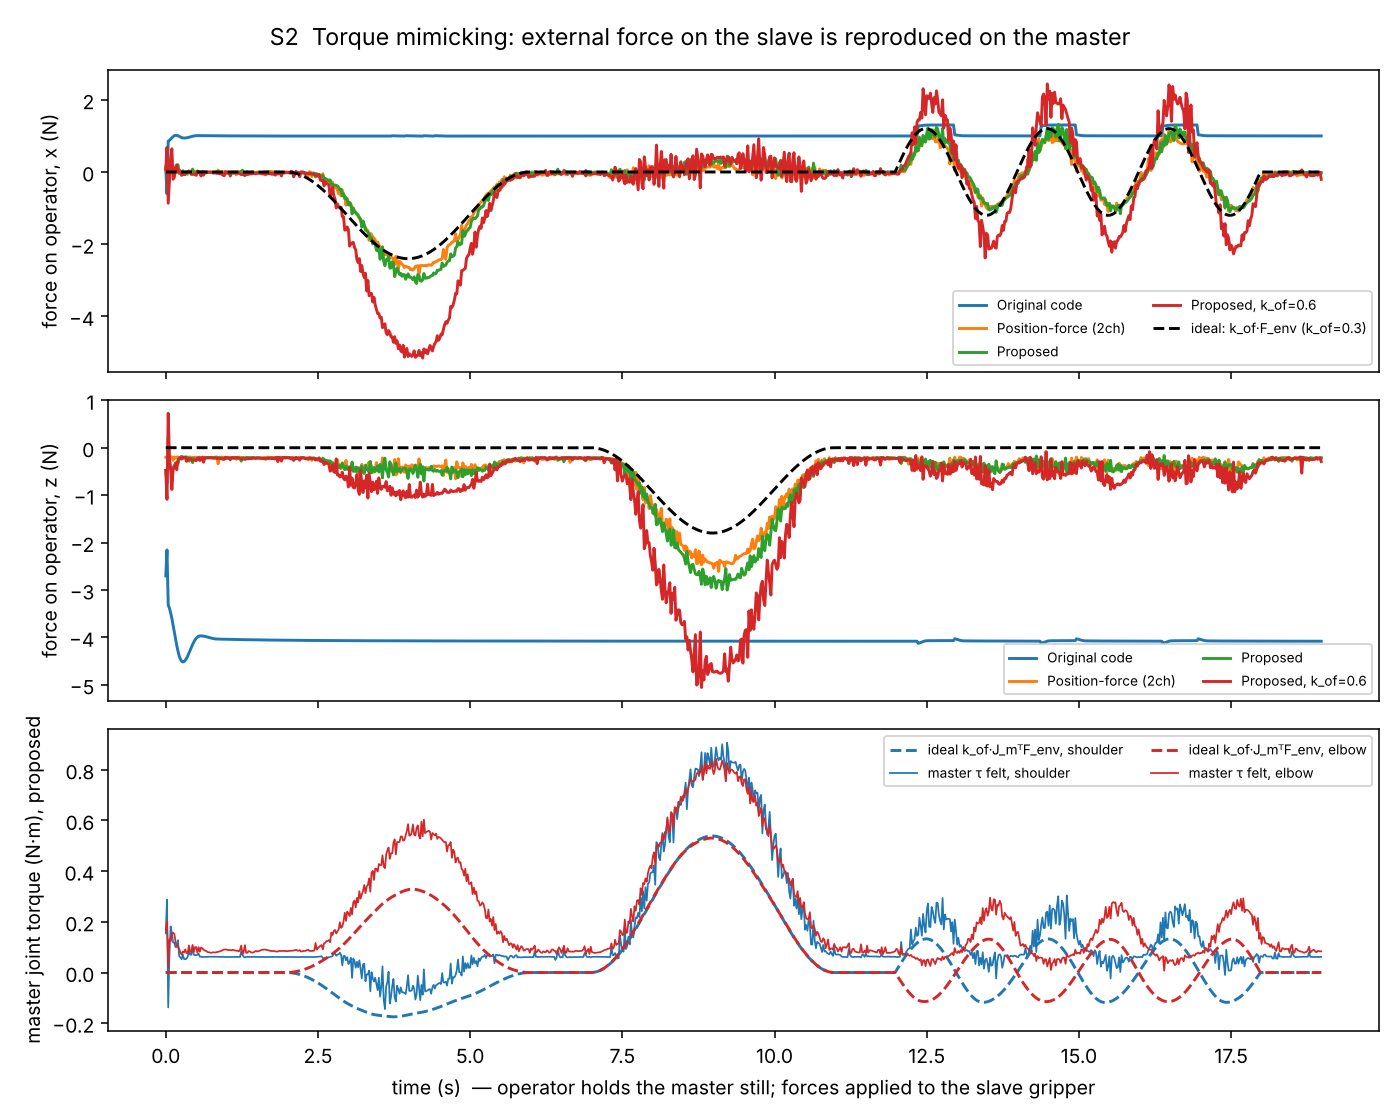
\includegraphics[width=\linewidth]{images/sim_torque_mimicking.png}
\caption{Simulated torque mimicking: forces applied to the slave gripper (top) and the force felt at the master for the original code, the position--force baseline, and the proposed controller. The operator holds the master still.}
\label{fig:sim_mimic}
\end{figure}

Fig.~\ref{fig:sim_stability} maps the maximum tracking error over force gain $k_{of}$ and one-way delay. The default $k_{of}=0.3$ is stable up to $60$\,ms; at $k_{of}=0.6$ the loop degrades from $20$\,ms. The energy tank reduces the worst case without delay (for $k_{of}=1.5$ from $1.99$ to $0.72$\,rad) but not reliably under delay, as expected from a tank that guards the master port only; delay-robust passivity needs a two-port tank or time-domain passivity control \cite{anderson1989,hannaford2002}. Measuring the real force path (calibration of $k_t$ with known masses, force against a scale) is part of the hardware protocol and is not claimed here.

\begin{figure}[t]
\centering
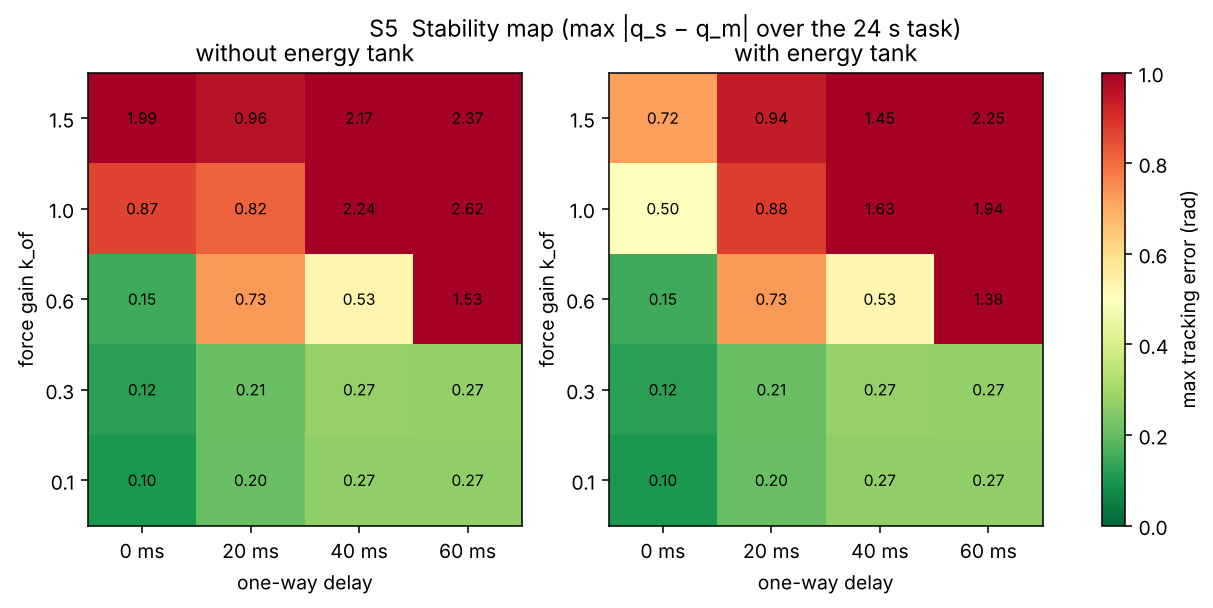
\includegraphics[width=\linewidth]{images/sim_stability_map.png}
\caption{Maximum tracking error versus force gain and delay without (left) and with (right) the energy tank, in simulation.}
\label{fig:sim_stability}
\end{figure}

\vspace{-0.35cm}
\subsection{Scalability to Learning-Based Control Pipelines}
% \vspace{-0.25cm}
The tracking and force-feedback behaviour above indicates that the testbed can serve as a platform for collecting data for data-driven control pipelines, but this has not yet been demonstrated with a trained policy. The testbed records synchronized trajectories, motor currents (as a proxy for contact force), and the commanded actions, together with the geometry of each camera, so that an operator who feels the environment's resistance can compensate for it naturally.
These episodes (HDF5 with the camera frames and calibration) can be fed to imitation learning or offline RL pipelines. Whether the operator's responses under force feedback help to close the sim-to-real gap in bimanual manipulation is a hypothesis for future experiments, not a result of this paper.

\subsection{Controller Parameter Tuning}
The simulator's plant is a mass--spring--damper ($m=1$\,kg, $b=0.5$\,N\,s/m, $k=2$\,N/m, step $10$\,ms, $|u|\le10$). A PID law is written as a control script whose parameters carry bounds, \texttt{Kp = 8; Ki = 0.5; Kd = 0.4;} with \texttt{@param} ranges $[0,50]$, $[0,10]$, and $[0,20]$. Differential evolution over these ranges with the ITAE objective moved the response from an overshoot of $36\%$ and an ITAE of $7.6$ to an overshoot of $2.5\%$ and an ITAE of $0.074$, with the gains ending at $K_p=45$, $K_i=6.0$, $K_d=9.4$. The proportional gain lies near its upper bound and the control saturates at $\pm10$ during the transient, so the result is limited by the actuator and by the search range, which is visible to the engineer before any hardware is touched. These numbers were obtained with a Python mirror of the MATLAB simulation function that is used for testing without a MATLAB licence; they are to be repeated in the MATLAB window before submission.

% \subsection{Controller Parameter Tuning and Performance \\Evaluation}
% % \vspace{-0.25cm}
% To demonstrate the testbed's capability for systematic parameter optimization, a second-order control system under different Proportional-Derivative (PD) controller configurations was tested. The simulation setup defined an initial position of $0$ with a velocity of $0.1$, aiming for a reference position of $1.0$ over a 10-second duration ($\Delta t = 0.01$\,s) with control saturation limits of $\pm 10$. 

% \begin{figure}[htbp]
% \centering
% \includegraphics[width=0.7\linewidth]{images/Para.jpeg}
% \caption{Comparison of system response, control effort, and tracking error during the PD controller parameter tuning process. \textcolor{green}{Green}: Initial Configuration;  \textcolor{blue}{Blue}: $K_p$ Optimised;  \textcolor{yellow!60!brown}{Yellow}: $K_p$ and $K_d$ Optimal}
% \label{fig:parameter_tuning}
% \end{figure}

% The experiment highlights the effect of progressively introducing proportional and derivative feedback Fig.~\ref{fig:parameter_tuning}:

%     \textit{Initial Configuration ($K_p = 0$, $K_d = 0$):} With no feedback control applied, the system acts as an unactuated setup, responding solely to its natural dynamics and initial positive velocity \( Green \). \\
%     \textit{Optimized Proportional Control ($K_p > 0$, $K_d = 0$):} Proportional control causes the actuator to generate effort proportional to the tracking error, driving the system rapidly toward the reference. \\
%     \textit{Optimized PD Control ($K_p > 0$, $K_d > 0$):} Derivative control introduces necessary damping by opposing rapid changes in the system state.

% The testbench facilitates quantitative controller tuning, by systematically sweeping controller gains within predefined search ranges, engineers can easily visualize the influence of proportional and derivative parameters on system dynamics and define their own configurations. This data-driven approach points out instability or excessive control effort, verify actuator limits, and achieve a stable balance between response speed and steady-state accuracy entirely in simulation. This framework reduces physical tuning time, prevents hardware stress, and ensures much safer and more reliable robotic operations prior to real-world deployment.

% The trajectory tracking performance of the proposed robotic control testbed was evaluated using a dataset comprising 7,691 synchronized samples collected at $50Hz$ during various bilateral teleoperation experiments. For each sample, the desired joint positions generated by the master RX-200 arm were recorded together with the corresponding joint positions measured on the slave VX-300S arm. These synchronized measurements enabled frame-by-frame computation of the tracking error for each joint. Since the master and slave grippers possess different physical dimensions and motion ranges, the gripper command was linearly interpolated to compensate for the difference in kinematic scaling.
% The trajectory tracking performance of the proposed control testbed was evaluated by collecting synchronised samples at $50Hz$ over a series of bilateral teleoperation tasks. For each sample, the desired joint angles of the RX-200 Arms commanded by the operator was recorded alongside the actual joint positions  executed by the VX-300s Arms, enabling frame by frame computation. The Gripper joint was linearly interpolated owing to the difference in kinematic scaling of the 2 Arms.

% Table~\ref{tab:tracking_metrics}. summarizes the tracking performance using the Root Mean Square Error (RMSE), Mean Absolute Error (MAE), maximum tracking error for each joint.

% \begin{table}[th]
% \centering
% \caption{Joint Tracking Performance Metrics}
% \label{tab:tracking_metrics}
% \resizebox{\columnwidth}{!}{%
% \begin{tabular}{lccc}
% \hline
% \textbf{Joint} & \textbf{RMSE (rad)} & \textbf{MAE (rad)} & \textbf{Max Error (rad)} \\
% \hline
% Waist & 0.2250 & 0.1355 & 1.2164 \\
% Shoulder & 0.2715 & 0.1800 & 1.0569 \\
% Elbow & 0.3609 & 0.2492 & 1.3315 \\
% Wrist Angle & 0.3152 & 0.1954 & 1.5555 \\
% Wrist Rotate & 0.5366 & 0.3736 & 1.4251 \\
% \hline
% \textbf{Overall} & \textbf{0.3418} & \textbf{0.2267} & \textbf{1.5555} \\
% \hline
% \end{tabular}%
% }
% \end{table}

% The trajectory tracking performance of the proposed robotic control testbed was evaluated to quantify the fidelity with which operator-generated motions on the master manipulator could be reproduced by the slave manipulator during bilateral teleoperation. The primary objective of this experiment was to assess the capability of the proposed framework to maintain accurate joint-space synchronization while operating under a real-time control loop, thereby validating its suitability for teleoperation, control algorithm development, and learning-based robotic applications.

% A series of representative bilateral teleoperation tasks involving free-space motion and continuous joint-space trajectories were performed using the RX-200 master arm and the VX-300S slave arm. Joint states from both manipulators were sampled synchronously at a control frequency of 50 Hz, ensuring temporal alignment between operator commands and the corresponding slave response. At each sampling instant, the desired joint positions generated by the master manipulator were recorded together with the actual joint positions measured from the slave manipulator. Since the master and slave employ different gripper mechanisms with distinct motion ranges, the gripper command was linearly interpolated to compensate for the difference in kinematic scaling, allowing meaningful comparison of the commanded and measured trajectories.

% The synchronized joint trajectories were subsequently analyzed offline to compute the instantaneous tracking error for each degree of freedom throughout the experiment. Standard trajectory tracking metrics, including the Root Mean Square Error (RMSE), Mean Absolute Error (MAE), and maximum absolute tracking error, were evaluated for every joint as well as over the complete dataset. These metrics provide complementary measures of average tracking accuracy, accumulated tracking deviation, and worst-case performance during teleoperation.

% The experiment was designed not only to evaluate the effectiveness of the proposed bilateral control framework but also to demonstrate the robustness of the developed testbed as a research platform. By maintaining synchronized acquisition of joint trajectories while supporting real-time communication between heterogeneous robotic manipulators, the framework enables quantitative benchmarking of control algorithms, generation of high-quality demonstration datasets for imitation and reinforcement learning, and seamless transition between simulation and physical hardware. The obtained results confirm that the proposed architecture is capable of reproducing operator motions with high fidelity, thereby establishing a reliable foundation for advanced robotic manipulation, shared autonomy, and data-driven control research.

% % \begin{table}[t]
% % \centering
% % \caption{Joint Tracking Performance Metrics}
% % \label{tab:tracking_metrics}
% % \resizebox{\columnwidth}{!}{%
% % \begin{tabular}{lccccc}
% % \hline
% % \textbf{Joint} & \textbf{RMSE} & \textbf{MAE} & \textbf{Max Error} & \textbf{P95 Error} & \textbf{Tracking Score} \\
% % \hline
% % Joint 0 & 0.2250 & 0.1355 & 1.2164 & 0.5239 & 0.8346 \\
% % Joint 1 & 0.2715 & 0.1800 & 1.0569 & 0.6420 & 0.8480 \\
% % Joint 2 & 0.3609 & 0.2492 & 1.3315 & 0.7961 & 0.7958 \\
% % Joint 3 & 0.3152 & 0.1954 & 1.5555 & 0.7102 & 0.7602 \\
% % Joint 4 & 0.5366 & 0.3736 & 1.4251 & 1.0301 & 0.3545 \\
% % \hline
% % \textbf{Overall} & \textbf{0.3418} & \textbf{0.2267} & \textbf{1.5555} & \textbf{0.7405} & \textbf{0.7186} \\
% % \hline
% % \end{tabular}%
% % }
% % \end{table}


% % The results demonstrate accurate trajectory reproduction across the first four joints, with RMSE values below 0.37 rad and tracking scores exceeding 0.76. Joint~4 exhibits comparatively larger errors, primarily due to differences in the end-effector kinematics and gripper scaling between the master and slave manipulators. Across all joints, the proposed framework achieved an overall RMSE of 0.3418 rad and an average tracking score of 0.7186, demonstrating reliable trajectory tracking suitable for bilateral teleoperation, control algorithm development, and data collection for learning-based robotic applications.

% % \section{Discussion}
% % \section{Discussion}
% % \label{sec:discussion}

% % \textbf{Should we remove this para as well? Again sounds like AI in his words} 
% % The experimental evaluation of the proposed bimanual bilateral teleoperation framework demonstrates its efficacy in bridging the gap between high-fidelity human inputs and low-power embedded hardware execution. 

% \subsection{Tracking Performance and Controller Efficacy}
% The plot in Fig. \ref{fig:tracking_plot}. highlights the actual and target trajectories. While minor transient latencies are observed during high-frequency directional shifts - a known constraint of executing optimization-based controllers. Furthermore, keeping the forearm-roll joint stationary provided a necessary kinematic constraint that noticeably improved the MPC solver's real-time convergence rate proving computationally expensive control loops can be efficiently deployed on accessible hardware without sacrificing operational fidelity.

% \begin{figure}[htbp]
%     \centering
%     \includegraphics[width=\linewidth]{images/tracking_plot.png}
%     \caption{Position tracking performance of the MPC controller}
%     \label{fig:tracking_plot}
% \end{figure}



% \subsection{Real-World Applicability and Scalability}
% The robust tracking capabilities showcased in the results validate this testbed for several critical real-world domains. In hazardous environments, such as explosive ordnance disposal (EOD) or nuclear waste sorting, the integration of bilateral force feedback allows operators to sense environmental resistance, preventing the crushing of volatile materials. Similarly, the system's ability to seamlessly log these synchronized high-fidelity trajectories as ROS bags provides a highly scalable pipeline for generating Imitation Learning and Reinforcement Learning (RL) datasets.

% % By capturing the natural compliance of human operators through the bilateral interface, the recorded data is vastly superior to rigid, one-way teleoperation data for training downstream AI policies. 

% Ultimately, this modular, ROS2-native framework provides researchers with an accessible yet rigorous foundation for prototyping complex bimanual manipulation algorithms before deployment on mission-critical industrial or surgical platforms.


% \section{Experiments and Evaluation}

% The trajectory tracking fidelity of the proposed robotic control testbed was evaluated to quantify the system's capacity to maintain precise joint-space synchronization under a real-time control loop. Experiments were conducted over a series of bilateral teleoperation tasks involving both free-space motion and continuous environmental interaction. During these tasks, the desired joint trajectories commanded by the operator via the RX-200 master manipulator were recorded alongside the actual joint positions executed by the VX-300s slave manipulators. 

% To ensure temporal alignment, the joint states from both heterogeneous arms were sampled synchronously at a control frequency of $50Hz$. Because the master and slave systems employ different gripper mechanisms with distinct kinematic scales and motion ranges, the gripper actuation commands were linearly interpolated. This normalization enabled a direct, frame-by-frame computation of the instantaneous tracking error for each degree of freedom.

% Table~\ref{tab:tracking_metrics} summarizes the system's tracking performance across the dataset, detailing the Root Mean Square Error (RMSE), Mean Absolute Error (MAE), and maximum absolute tracking error for each joint. 

% \begin{table}[th]
% \centering
% \caption{Joint Tracking Performance Metrics}
% \label{tab:tracking_metrics}
% \resizebox{\columnwidth}{!}{%
% \begin{tabular}{lccc}
% \hline
% \textbf{Joint} & \textbf{RMSE (rad)} & \textbf{MAE (rad)} & \textbf{Max Error (rad)} \\
% \hline
% Waist & 0.2250 & 0.1355 & 1.2164 \\
% Shoulder & 0.2715 & 0.1800 & 1.0569 \\
% Elbow & 0.3609 & 0.2492 & 1.3315 \\
% Wrist Angle & 0.3152 & 0.1954 & 1.5555 \\
% Wrist Rotate & 0.5366 & 0.3736 & 1.4251 \\
% \hline
% \textbf{Overall} & \textbf{0.3418} & \textbf{0.2267} & \textbf{1.5555} \\
% \hline
% \end{tabular}%
% }
% \end{table}

% \subsection{Tracking Performance and Controller Efficacy}
% As detailed in Table~\ref{tab:tracking_metrics}, the proximal joints (Waist, Shoulder) exhibit lower tracking errors compared to the distal joints (Wrist Rotate). This variance is expected in multi-link manipulators, as kinematic errors naturally compound along the kinematic chain. The overall position tracking performance of the underlying Model Predictive Control (MPC) formulation is visualized in Fig.~\ref{fig:tracking_plot}, mapping actual versus target trajectories.

% While the system successfully maintains low-deviation synchronization (Overall RMSE of $0.3418$ rad), minor transient latencies are observable during high-frequency directional shifts. This is a known, inherent constraint of executing constrained optimization-based controllers, where the solver must compute optimal torques over a predictive horizon within the strict $20ms$ window of the $50Hz$ control loop. To mitigate this computational overhead and guarantee real-time convergence, the forearm-roll joint was kinematically constrained. By holding this joint stationary, the state-space dimensionality of the MPC solver was effectively reduced. This deliberate constraint noticeably accelerated the optimization cycle, proving that computationally demanding control architectures can be efficiently deployed on accessible hardware without sacrificing the operational workspace required for complex manipulation.

% \begin{figure}[htbp]
%     \centering
%     \includegraphics[width=\linewidth]{images/tracking_plot.png}
%     \caption{Position tracking performance of the MPC controller during continuous teleoperation.}
%     \label{fig:tracking_plot}
% \end{figure}

% \subsection{Scalability to Learning-Based Control Pipelines}
% Beyond validating the MPC architecture, the robust tracking capabilities established here demonstrate the testbed's viability as a high-fidelity data acquisition pipeline for data-driven robotics. Standard unilateral teleoperation often yields rigid, open-loop demonstrations that fail to capture environmental contact dynamics. In contrast, integrating bilateral force feedback allows human operators to naturally sense resistance and exhibit corrective compliance. 

% By seamlessly logging these synchronized, force-responsive trajectories as ROS2 bags, this framework serves as an optimized engine for generating high-quality datasets for Imitation Learning (IL) and offline Reinforcement Learning (RL). The ability to capture the natural compliance of human operators significantly bridges the sim-to-real gap, providing researchers with a rigorous hardware foundation for prototyping and deploying complex bimanual manipulation policies.

% \vspace{-0.25cm}
\section{Conclusion and Future Work}
% \vspace{-0.35cm}
The platform integrates bilateral teleoperation, control development, and a geometry-aware data pipeline for multi-arm setups. On a bimanual Interbotix XS setup, the initial implementation tracked with an overall RMSE of 0.3583\,rad without force-torque sensors. The analysis of that result led to a revised controller (momentum observer, exact admittance discretisation, offset-free position MPC, Jacobian force mapping, energy tank) that is evaluated here in a MuJoCo model of the same arms, where it removes the dominant lag and reproduces applied forces at the master. Its performance on the real arms, and with a real force path, is not yet measured; a protocol for those measurements is part of the repository. The open design, which delegates algorithm and library selection to the user while providing a consistent data interface, keeps MERLIN compatible with evolving RL methods, simulation engines, and robot hardware.
\hspace{1em}Future work will focus on four directions. First, measuring the revised controller on the real arms (calibration of the torque constants, identification of the servo position loop, force path against a scale). Second, delay-robust passivity with a two-port energy tank, and collision detection in the safety layer. Third, touch-based haptic feedback and additional sensing, which the episode schema is meant to accommodate. Fourth, extending the teleoperation input modalities to include exoskeleton-based interfaces for higher-fidelity human motion capture.

% \section{MATH}

% Before you begin to format your paper, first write and save the content as a separate text file. Keep your text and graphic files separate until after the text has been formatted and styled. Do not use hard tabs, and limit use of hard returns to only one return at the end of a paragraph. Do not add any kind of pagination anywhere in the paper. Do not number text heads-the template will do that for you.

% Finally, complete content and organizational editing before formatting. Please take note of the following items when proofreading spelling and grammar:

% \subsection{Abbreviations and Acronyms} Define abbreviations and acronyms the first time they are used in the text, even after they have been defined in the abstract. Abbreviations such as IEEE, SI, MKS, CGS, sc, dc, and rms do not have to be defined. Do not use abbreviations in the title or heads unless they are unavoidable.

% \subsection{Units}

% \begin{itemize}

% \item Use either SI (MKS) or CGS as primary units. (SI units are encouraged.) English units may be used as secondary units (in parentheses). An exception would be the use of English units as identifiers in trade, such as Ò3.5-inch disk driveÓ.
% \item Avoid combining SI and CGS units, such as current in amperes and magnetic field in oersteds. This often leads to confusion because equations do not balance dimensionally. If you must use mixed units, clearly state the units for each quantity that you use in an equation.
% \item Do not mix complete spellings and abbreviations of units: ÒWb/m2Ó or Òwebers per square meterÓ, not Òwebers/m2Ó.  Spell out units when they appear in text: Ò. . . a few henriesÓ, not Ò. . . a few HÓ.
% \item Use a zero before decimal points: Ò0.25Ó, not Ò.25Ó. Use Òcm3Ó, not ÒccÓ. (bullet list)

% \end{itemize}


% \subsection{Equations}

% The equations are an exception to the prescribed specifications of this template. You will need to determine whether or not your equation should be typed using either the Times New Roman or the Symbol font (please no other font). To create multileveled equations, it may be necessary to treat the equation as a graphic and insert it into the text after your paper is styled. Number equations consecutively. Equation numbers, within parentheses, are to position flush right, as in (1), using a right tab stop. To make your equations more compact, you may use the solidus ( / ), the exp function, or appropriate exponents. Italicize Roman symbols for quantities and variables, but not Greek symbols. Use a long dash rather than a hyphen for a minus sign. Punctuate equations with commas or periods when they are part of a sentence, as in

% $$
% \alpha + \beta = \chi \eqno{(1)}
% $$

% Note that the equation is centered using a center tab stop. Be sure that the symbols in your equation have been defined before or immediately following the equation. Use Ò(1)Ó, not ÒEq. (1)Ó or Òequation (1)Ó, except at the beginning of a sentence: ÒEquation (1) is . . .Ó

% \subsection{Some Common Mistakes}
% \begin{itemize}


% \item The word ÒdataÓ is plural, not singular.
% \item The subscript for the permeability of vacuum ?0, and other common scientific constants, is zero with subscript formatting, not a lowercase letter ÒoÓ.
% \item In American English, commas, semi-/colons, periods, question and exclamation marks are located within quotation marks only when a complete thought or name is cited, such as a title or full quotation. When quotation marks are used, instead of a bold or italic typeface, to highlight a word or phrase, punctuation should appear outside of the quotation marks. A parenthetical phrase or statement at the end of a sentence is punctuated outside of the closing parenthesis (like this). (A parenthetical sentence is punctuated within the parentheses.)
% \item A graph within a graph is an ÒinsetÓ, not an ÒinsertÓ. The word alternatively is preferred to the word ÒalternatelyÓ (unless you really mean something that alternates).
% \item Do not use the word ÒessentiallyÓ to mean ÒapproximatelyÓ or ÒeffectivelyÓ.
% \item In your paper title, if the words Òthat usesÓ can accurately replace the word ÒusingÓ, capitalize the ÒuÓ; if not, keep using lower-cased.
% \item Be aware of the different meanings of the homophones ÒaffectÓ and ÒeffectÓ, ÒcomplementÓ and ÒcomplimentÓ, ÒdiscreetÓ and ÒdiscreteÓ, ÒprincipalÓ and ÒprincipleÓ.
% \item Do not confuse ÒimplyÓ and ÒinferÓ.
% \item The prefix ÒnonÓ is not a word; it should be joined to the word it modifies, usually without a hyphen.
% \item There is no period after the ÒetÓ in the Latin abbreviation Òet al.Ó.
% \item The abbreviation Òi.e.Ó means Òthat isÓ, and the abbreviation Òe.g.Ó means Òfor exampleÓ.

% \end{itemize}


% \section{USING THE TEMPLATE}

% Use this sample document as your LaTeX source file to create your document. Save this file as {\bf root.tex}. You have to make sure to use the cls file that came with this distribution. If you use a different style file, you cannot expect to get required margins. Note also that when you are creating your out PDF file, the source file is only part of the equation. {\it Your \TeX\ $\rightarrow$ PDF filter determines the output file size. Even if you make all the specifications to output a letter file in the source - if your filter is set to produce A4, you will only get A4 output. }

% It is impossible to account for all possible situation, one would encounter using \TeX. If you are using multiple \TeX\ files you must make sure that the ``MAIN`` source file is called root.tex - this is particularly important if your conference is using PaperPlaza's built in \TeX\ to PDF conversion tool.

% \subsection{Headings, etc}

% Text heads organize the topics on a relational, hierarchical basis. For example, the paper title is the primary text head because all subsequent material relates and elaborates on this one topic. If there are two or more sub-topics, the next level head (uppercase Roman numerals) should be used and, conversely, if there are not at least two sub-topics, then no subheads should be introduced. Styles named ÒHeading 1Ó, ÒHeading 2Ó, ÒHeading 3Ó, and ÒHeading 4Ó are prescribed.

% \subsection{Figures and Tables}

% Positioning Figures and Tables: Place figures and tables at the top and bottom of columns. Avoid placing them in the middle of columns. Large figures and tables may span across both columns. Figure captions should be below the figures; table heads should appear above the tables. Insert figures and tables after they are cited in the text. Use the abbreviation ÒFig. 1Ó, even at the beginning of a sentence.

% \begin{table}[h]
% \caption{An Example of a Table}
% \label{table_example}
% \begin{center}
% \begin{tabular}{|c||c|}
% \hline
% One & Two\\
% \hline
% Three & Four\\
% \hline
% \end{tabular}
% \end{center}
% \end{table}


%    \begin{figure}[thpb]
%       \centering
%       \framebox{\parbox{3in}{We suggest that you use a text box to insert a graphic (which is ideally a 300 dpi TIFF or EPS file, with all fonts embedded) because, in an document, this method is somewhat more stable than directly inserting a picture.
% }}
%       %\includegraphics[scale=1.0]{figurefile}
%       \caption{Inductance of oscillation winding on amorphous
%        magnetic core versus DC bias magnetic field}
%       \label{figurelabel}
%    \end{figure}
   

% Figure Labels: Use 8 point Times New Roman for Figure labels. Use words rather than symbols or abbreviations when writing Figure axis labels to avoid confusing the reader. As an example, write the quantity ÒMagnetizationÓ, or ÒMagnetization, MÓ, not just ÒMÓ. If including units in the label, present them within parentheses. Do not label axes only with units. In the example, write ÒMagnetization (A/m)Ó or ÒMagnetization {A[m(1)]}Ó, not just ÒA/mÓ. Do not label axes with a ratio of quantities and units. For example, write ÒTemperature (K)Ó, not ÒTemperature/K.Ó

% \section{CONCLUSIONS}

% A conclusion section is not required. Although a conclusion may review the main points of the paper, do not replicate the abstract as the conclusion. A conclusion might elaborate on the importance of the work or suggest applications and extensions. 

\addtolength{\textheight}{-14.5cm}   % This command serves to balance the column lengths
                                  % on the last page of the document manually. It shortens
                                  % the textheight of the last page by a suitable amount.
                                  % This command does not take effect until the next page
                                  % so it should come on the page before the last. Make
                                  % sure that you do not shorten the textheight too much.

%%%%%%%%%%%%%%%%%%%%%%%%%%%%%%%%%%%%%%%%%%%%%%%%%%%%%%%%%%%%%%%%%%%%%%%%%%%%%%%%



%%%%%%%%%%%%%%%%%%%%%%%%%%%%%%%%%%%%%%%%%%%%%%%%%%%%%%%%%%%%%%%%%%%%%%%%%%%%%%%%



%%%%%%%%%%%%%%%%%%%%%%%%%%%%%%%%%%%%%%%%%%%%%%%%%%%%%%%%%%%%%%%%%%%%%%%%%%%%%%%%
% \section*{APPENDIX}

% Appendixes should appear before the acknowledgment.

% \section*{ACKNOWLEDGMENT}

% The preferred spelling of the word ÒacknowledgmentÓ in America is without an ÒeÓ after the ÒgÓ. Avoid the stilted expression, ÒOne of us (R. B. G.) thanks . . .Ó  Instead, try ÒR. B. G. thanksÓ. Put sponsor acknowledgments in the unnumbered footnote on the first page.



% %%%%%%%%%%%%%%%%%%%%%%%%%%%%%%%%%%%%%%%%%%%%%%%%%%%%%%%%%%%%%%%%%%%%%%%%%%%%%%%%

% References are important to the reader; therefore, each citation must be complete and correct. If at all possible, references should be commonly available publications.



% \begin{thebibliography}{99}

% \bibitem{c1} G. O. Young, ÒSynthetic structure of industrial plastics (Book style with paper title and editor),Ó 	in Plastics, 2nd ed. vol. 3, J. Peters, Ed.  New York: McGraw-Hill, 1964, pp. 15Ð64.
% \bibitem{c2} W.-K. Chen, Linear Networks and Systems (Book style).	Belmont, CA: Wadsworth, 1993, pp. 123Ð135.
% \bibitem{c3} H. Poor, An Introduction to Signal Detection and Estimation.   New York: Springer-Verlag, 1985, ch. 4.
% \bibitem{c4} B. Smith, ÒAn approach to graphs of linear forms (Unpublished work style),Ó unpublished.
% \bibitem{c5} E. H. Miller, ÒA note on reflector arrays (Periodical styleÑAccepted for publication),Ó IEEE Trans. Antennas Propagat., to be publised.
% \bibitem{c6} J. Wang, ÒFundamentals of erbium-doped fiber amplifiers arrays (Periodical styleÑSubmitted for publication),Ó IEEE J. Quantum Electron., submitted for publication.
% \bibitem{c7} C. J. Kaufman, Rocky Mountain Research Lab., Boulder, CO, private communication, May 1995.
% \bibitem{c8} Y. Yorozu, M. Hirano, K. Oka, and Y. Tagawa, ÒElectron spectroscopy studies on magneto-optical media and plastic substrate interfaces(Translation Journals style),Ó IEEE Transl. J. Magn.Jpn., vol. 2, Aug. 1987, pp. 740Ð741 [Dig. 9th Annu. Conf. Magnetics Japan, 1982, p. 301].
% \bibitem{c9} M. Young, The Techincal Writers Handbook.  Mill Valley, CA: University Science, 1989.
% \bibitem{c10} J. U. Duncombe, ÒInfrared navigationÑPart I: An assessment of feasibility (Periodical style),Ó IEEE Trans. Electron Devices, vol. ED-11, pp. 34Ð39, Jan. 1959.
% \bibitem{c11} S. Chen, B. Mulgrew, and P. M. Grant, ÒA clustering technique for digital communications channel equalization using radial basis function networks,Ó IEEE Trans. Neural Networks, vol. 4, pp. 570Ð578, July 1993.
% \bibitem{c12} R. W. Lucky, ÒAutomatic equalization for digital communication,Ó Bell Syst. Tech. J., vol. 44, no. 4, pp. 547Ð588, Apr. 1965.
% \bibitem{c13} S. P. Bingulac, ÒOn the compatibility of adaptive controllers (Published Conference Proceedings style),Ó in Proc. 4th Annu. Allerton Conf. Circuits and Systems Theory, New York, 1994, pp. 8Ð16.
% \bibitem{c14} G. R. Faulhaber, ÒDesign of service systems with priority reservation,Ó in Conf. Rec. 1995 IEEE Int. Conf. Communications, pp. 3Ð8.
% \bibitem{c15} W. D. Doyle, ÒMagnetization reversal in films with biaxial anisotropy,Ó in 1987 Proc. INTERMAG Conf., pp. 2.2-1Ð2.2-6.
% \bibitem{c16} G. W. Juette and L. E. Zeffanella, ÒRadio noise currents n short sections on bundle conductors (Presented Conference Paper style),Ó presented at the IEEE Summer power Meeting, Dallas, TX, June 22Ð27, 1990, Paper 90 SM 690-0 PWRS.
% \bibitem{c17} J. G. Kreifeldt, ÒAn analysis of surface-detected EMG as an amplitude-modulated noise,Ó presented at the 1989 Int. Conf. Medicine and Biological Engineering, Chicago, IL.
% \bibitem{c18} J. Williams, ÒNarrow-band analyzer (Thesis or Dissertation style),Ó Ph.D. dissertation, Dept. Elect. Eng., Harvard Univ., Cambridge, MA, 1993. 
% \bibitem{c19} N. Kawasaki, ÒParametric study of thermal and chemical nonequilibrium nozzle flow,Ó M.S. thesis, Dept. Electron. Eng., Osaka Univ., Osaka, Japan, 1993.
% \bibitem{c20} J. P. Wilkinson, ÒNonlinear resonant circuit devices (Patent style),Ó U.S. Patent 3 624 12, July 16, 1990. 






% \end{thebibliography}
\bibliographystyle{IEEEtranS} 
\bibliography{IEEEfull,references,references_additions}
\end{document}
